% Add this at the top of your main document if not already present
% \usepackage{float}

\section{Introduction}
\noindent
The Candidate Platform has been successfully implemented and deployed, providing a comprehensive solution for VOID Digital Agency's intern recruitment process. This chapter presents a detailed walkthrough of the platform's functionality, demonstrating how it streamlines the entire recruitment workflow from job posting to final candidate selection.

\section{Project Results and Showcase}



\subsection{Main Page Components}
\noindent
The main page showcases key information through various components:

\begin{figure}[H]
    \centering
    \makebox[\textwidth]{%
        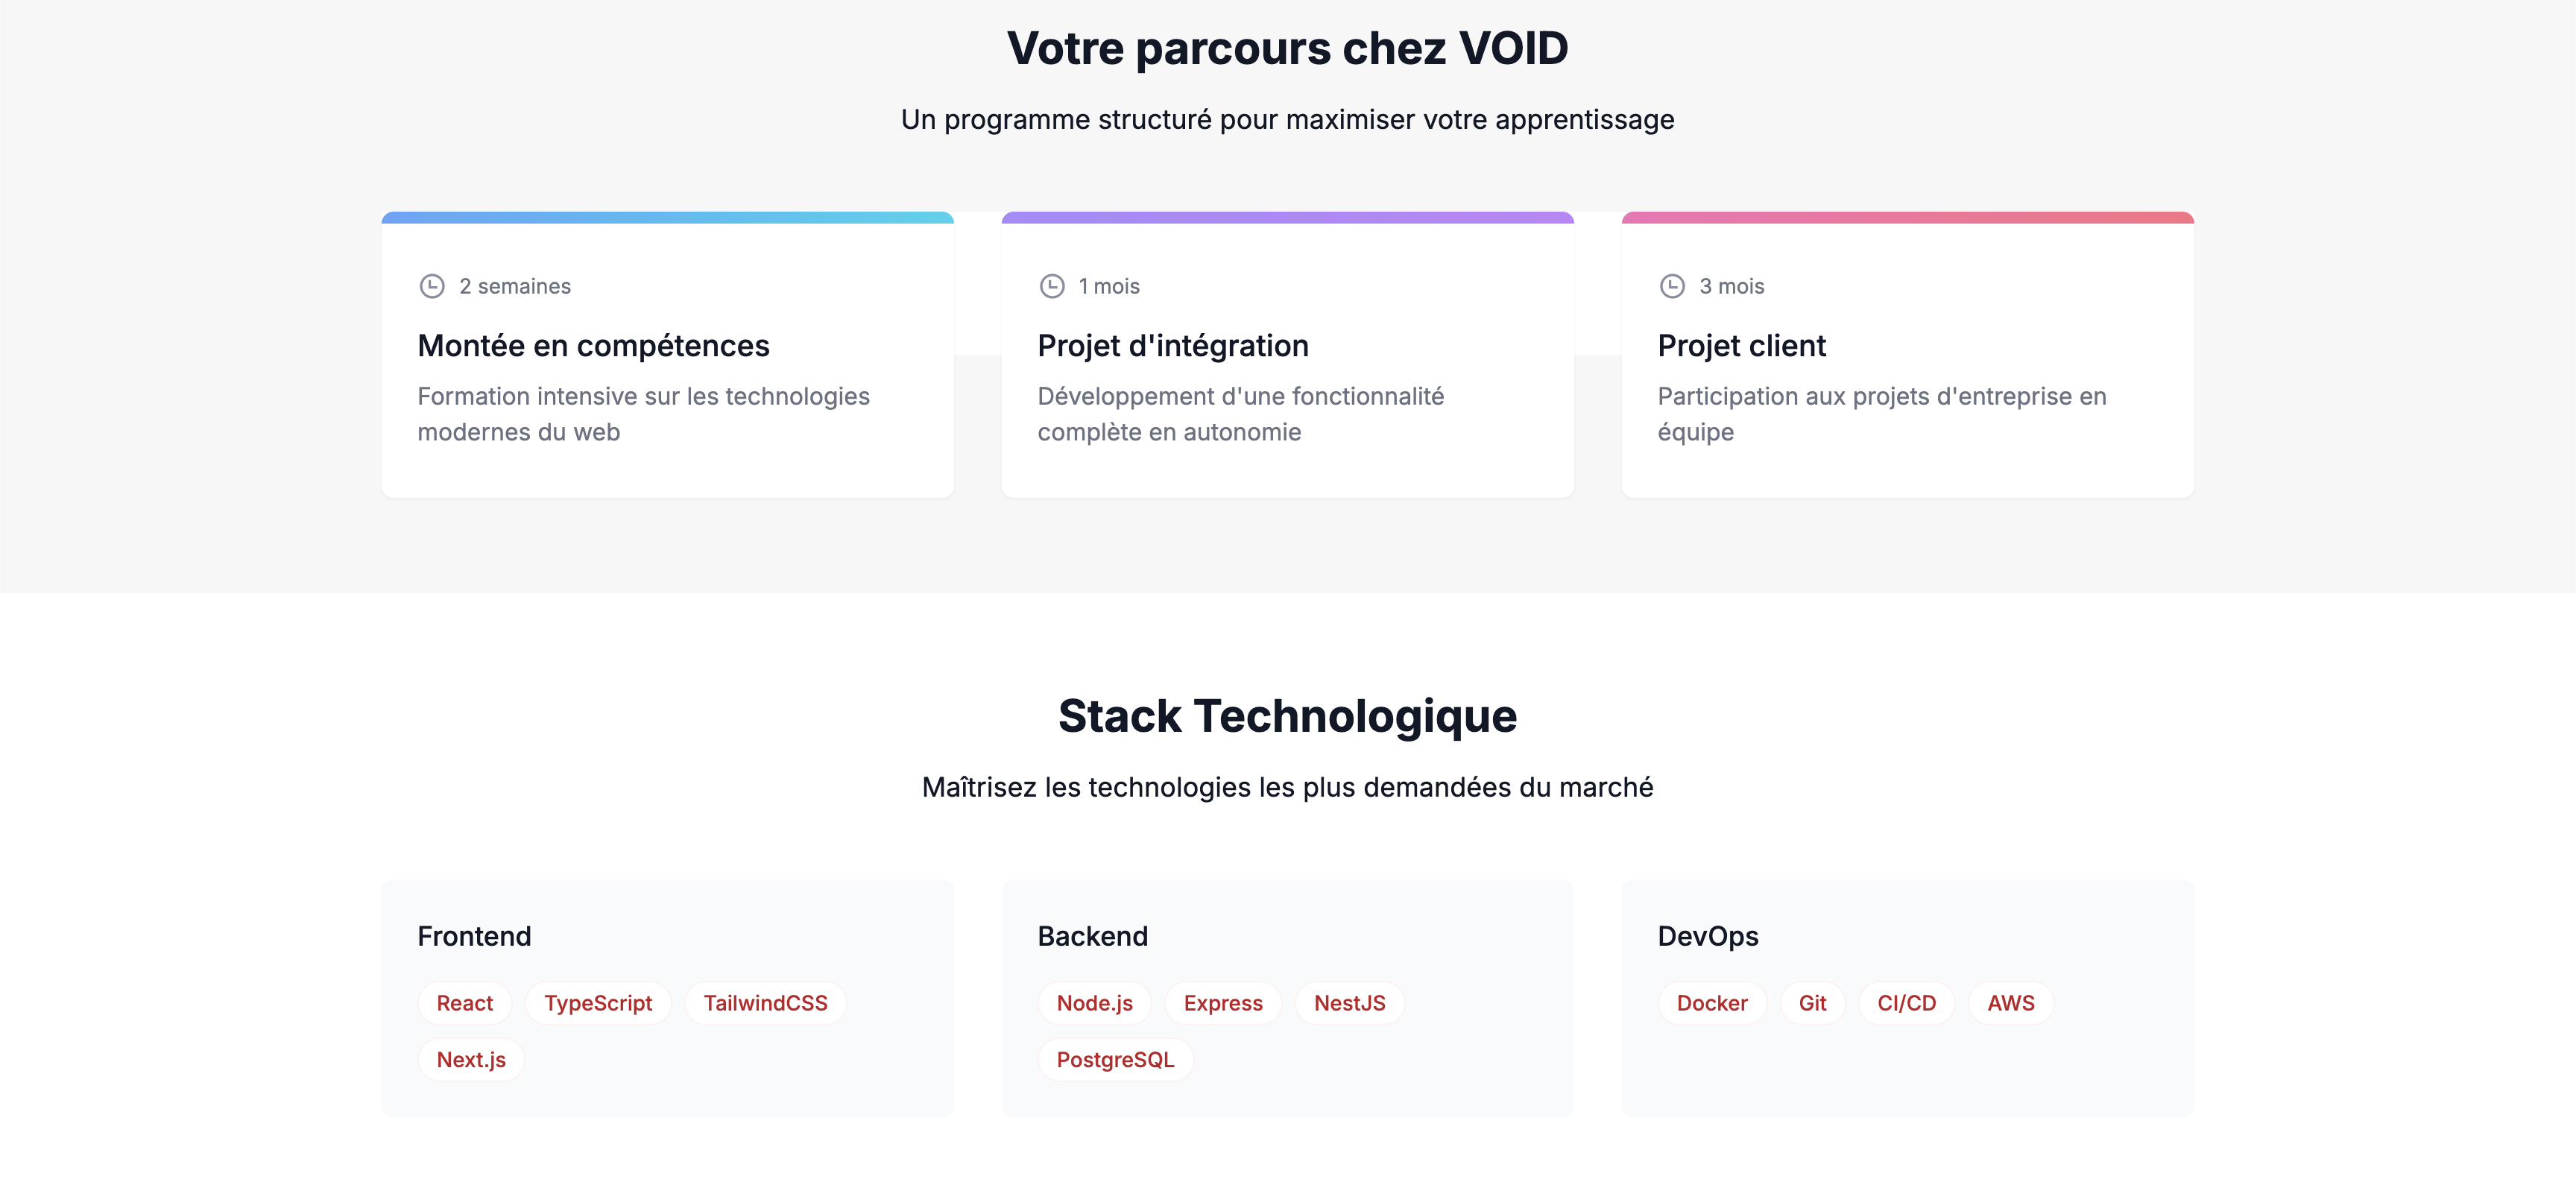
\includegraphics[width=1.1\textwidth]{images/Screenshot-intern-main-page-section}%
    }
    \caption{Main Page Cards Display}
    \label{fig:main_cards}
\end{figure}

\begin{figure}[H]
    \centering
    \makebox[\textwidth]{%
        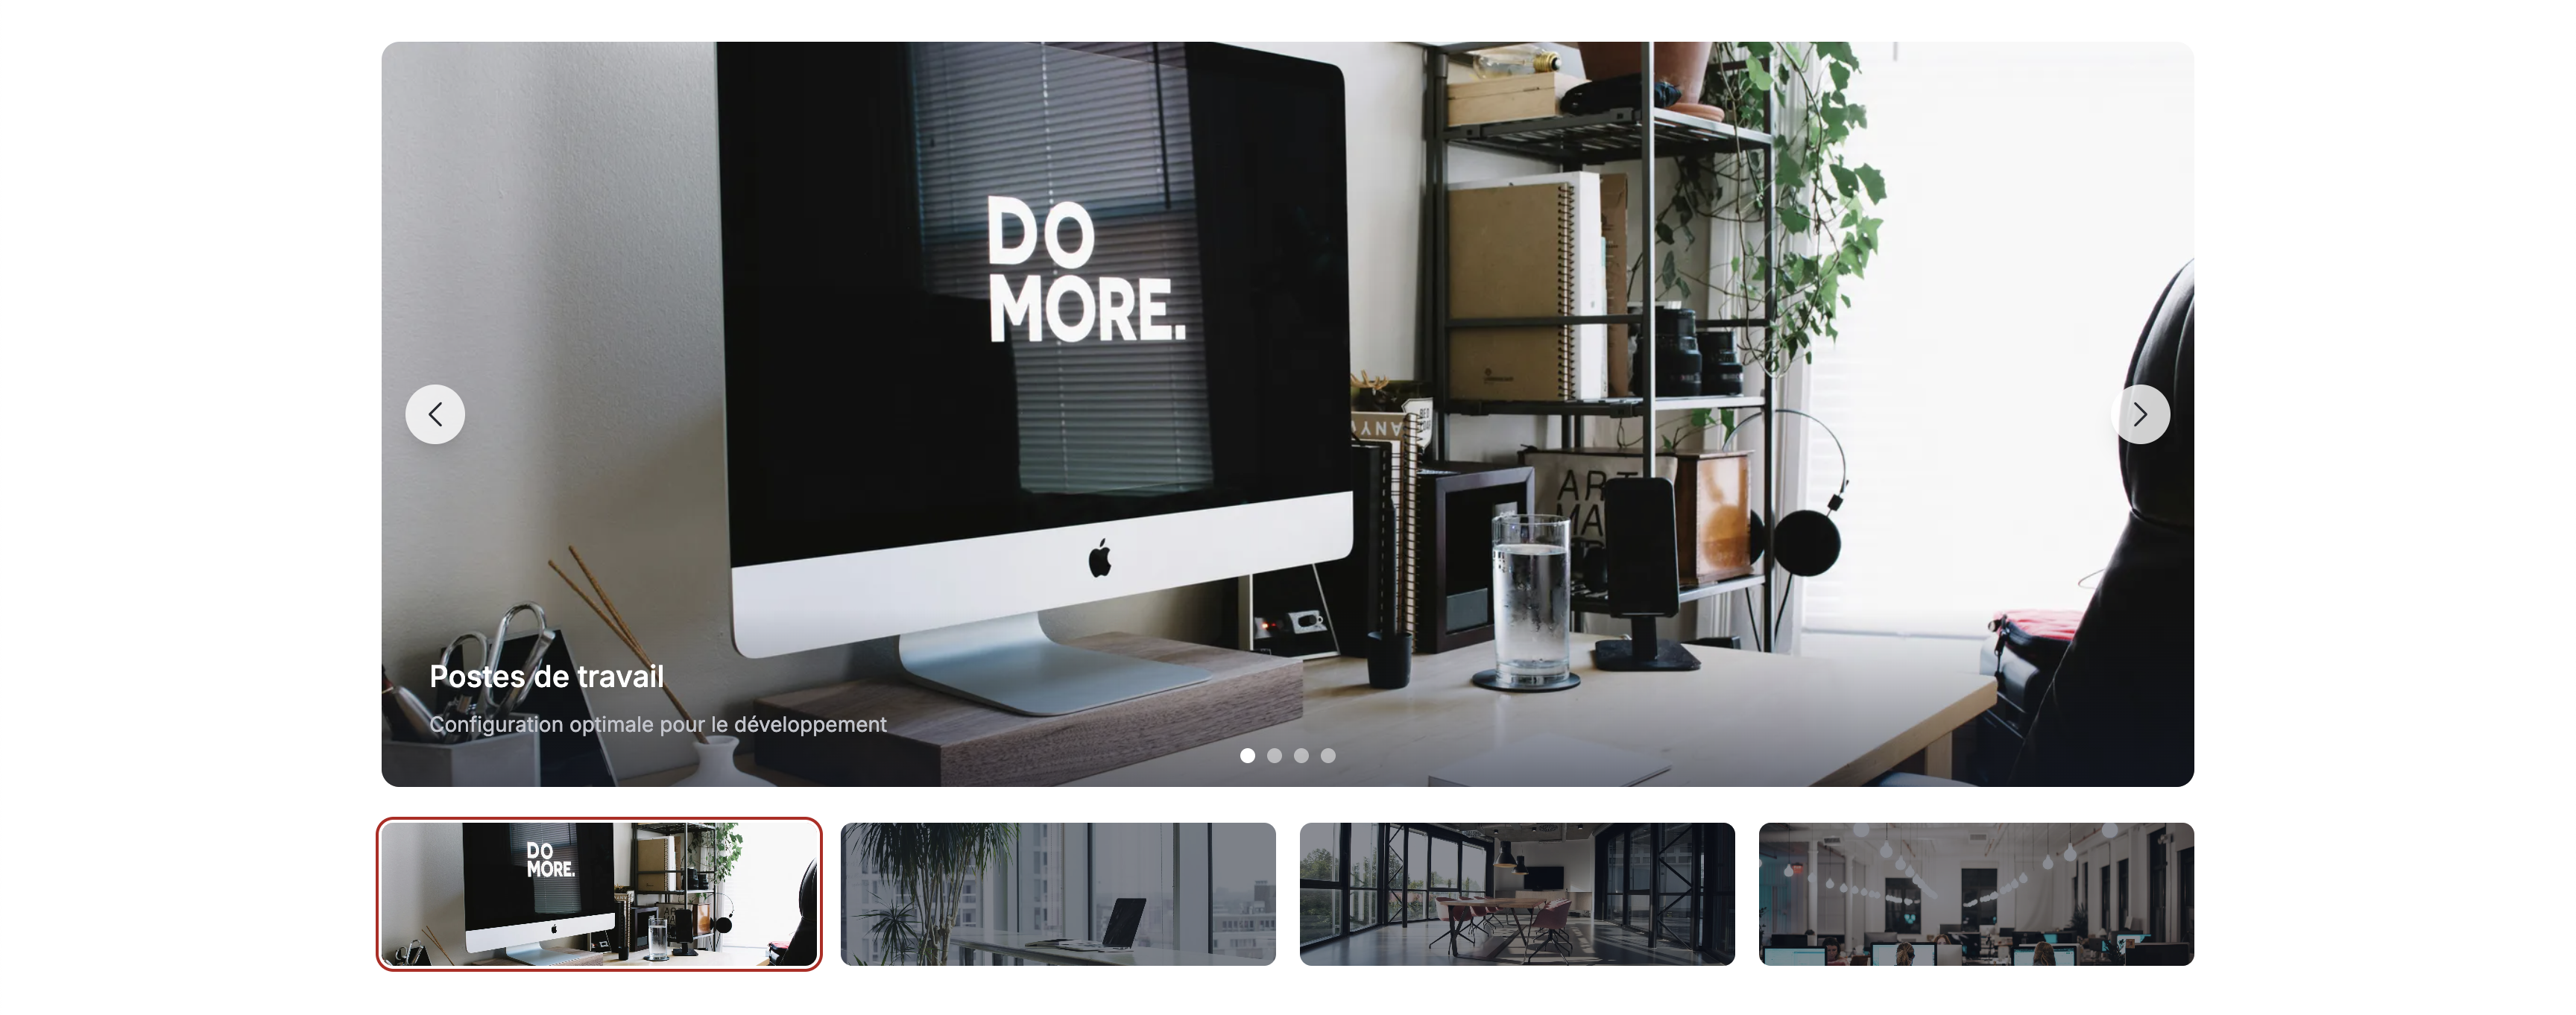
\includegraphics[width=1.1\textwidth]{images/Screenshot-sledr}%
    }
    \caption{Main Page Slider}
    \label{fig:main_slider}
\end{figure}

\subsection{Intern Dashboard Overview}
\noindent
The intern dashboard provides a comprehensive overview of the internship experience with clear navigation and timeline tracking:

\begin{figure}[H]
    \centering
    \makebox[\textwidth]{%
        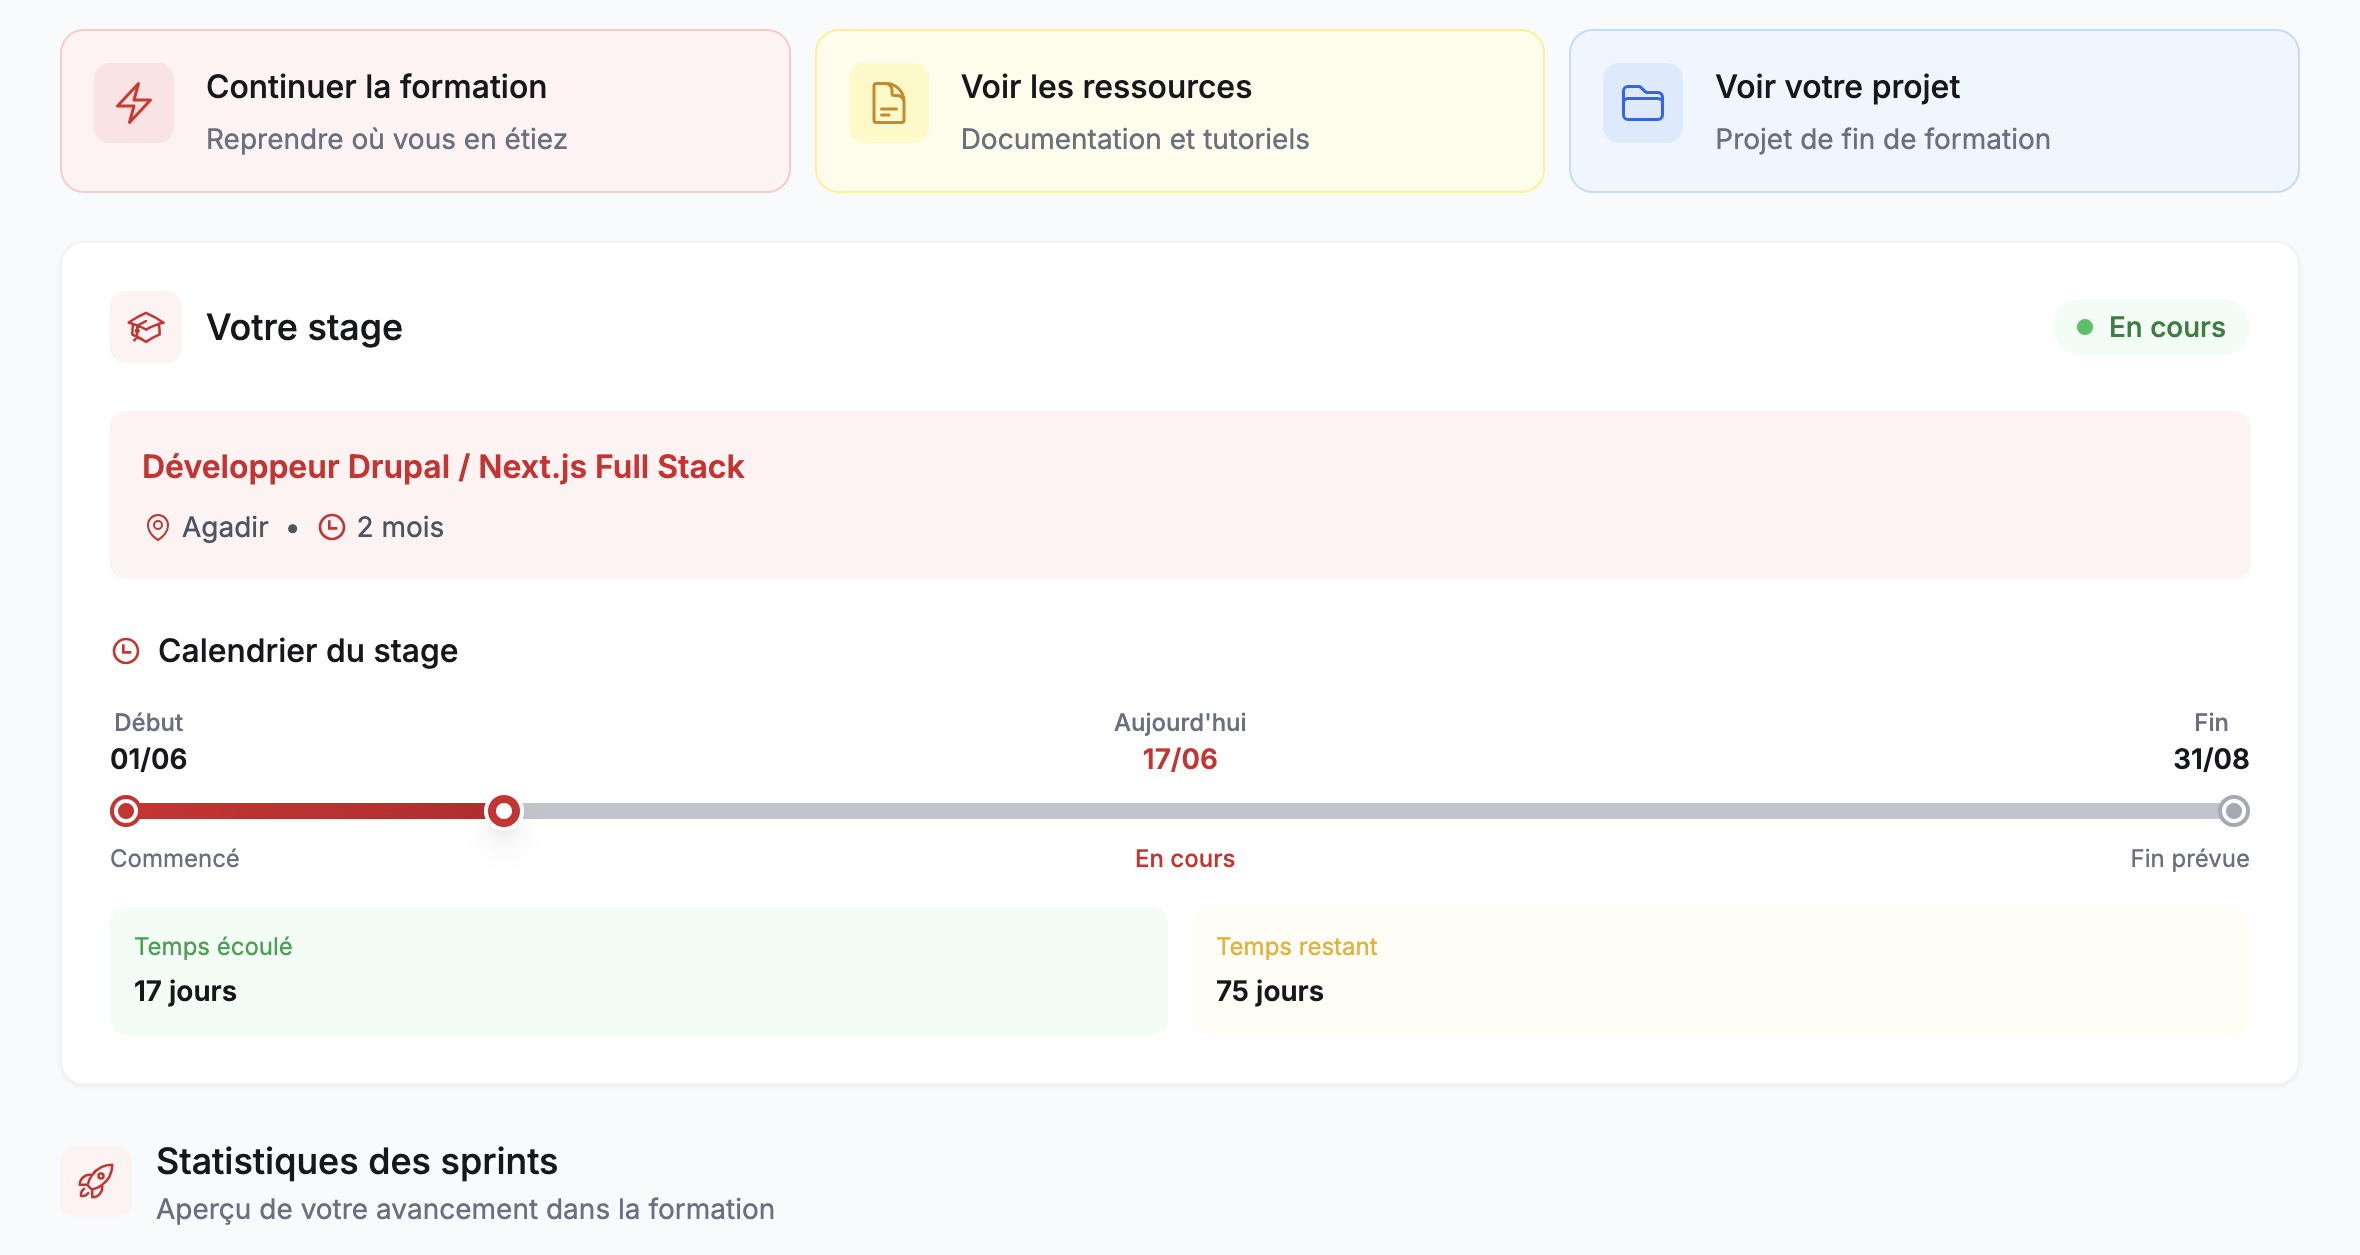
\includegraphics[width=1.1\textwidth]{images/image-dash-1}%
    }
    \caption{Intern Dashboard - Access and Navigation with Timeline}
    \label{fig:intern_dashboard}
\end{figure}

This dashboard illustrates:
\begin{itemize}
    \item Complete internship timeline and progress
    \item Easy navigation to all platform features
    \item Current status and upcoming milestones
    \item Quick access to assigned tasks and resources
\end{itemize}

\subsection{Sprint Statistics Dashboard}
\noindent
A dedicated sprint statistics dashboard provides detailed insights into sprint performance and management:

\begin{figure}[H]
    \centering
    \makebox[\textwidth]{%
        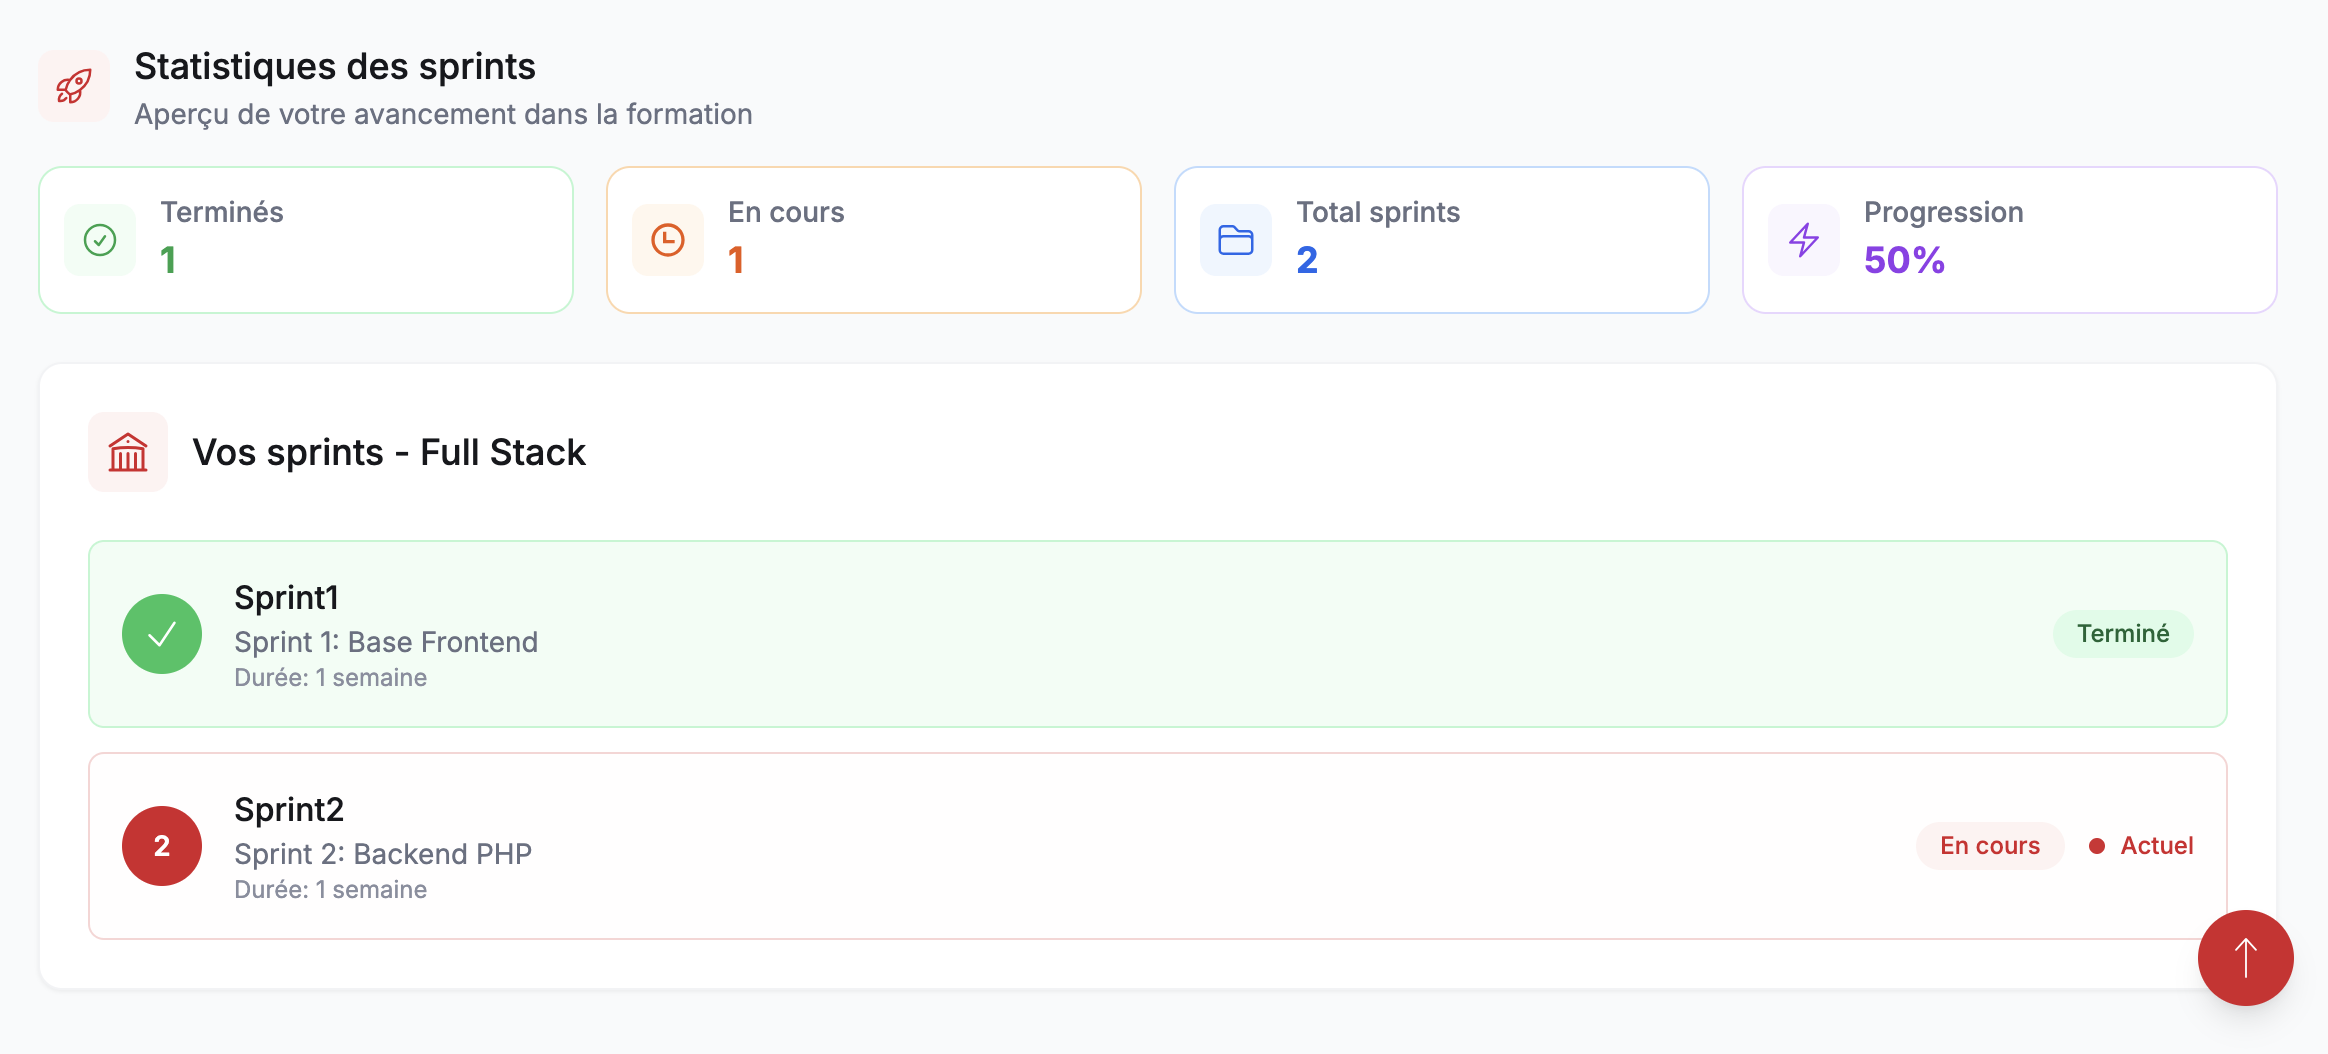
\includegraphics[width=1.1\textwidth]{images/image-dash-2}%
    }
    \caption{Sprint Statistics and Sprint Listings Dashboard}
    \label{fig:sprint_dashboard}
\end{figure}

The sprint dashboard displays:
\begin{itemize}
    \item Comprehensive sprint statistics and metrics
    \item Small sprint listings with key information
    \item Progress tracking across all sprints
    \item Performance analytics and completion rates
\end{itemize}

\subsection{Intern Sprint Management}
\noindent
Each intern has access to their assigned sprints with clear progress tracking:

\begin{figure}[H]
    \centering
    \makebox[\textwidth]{%
        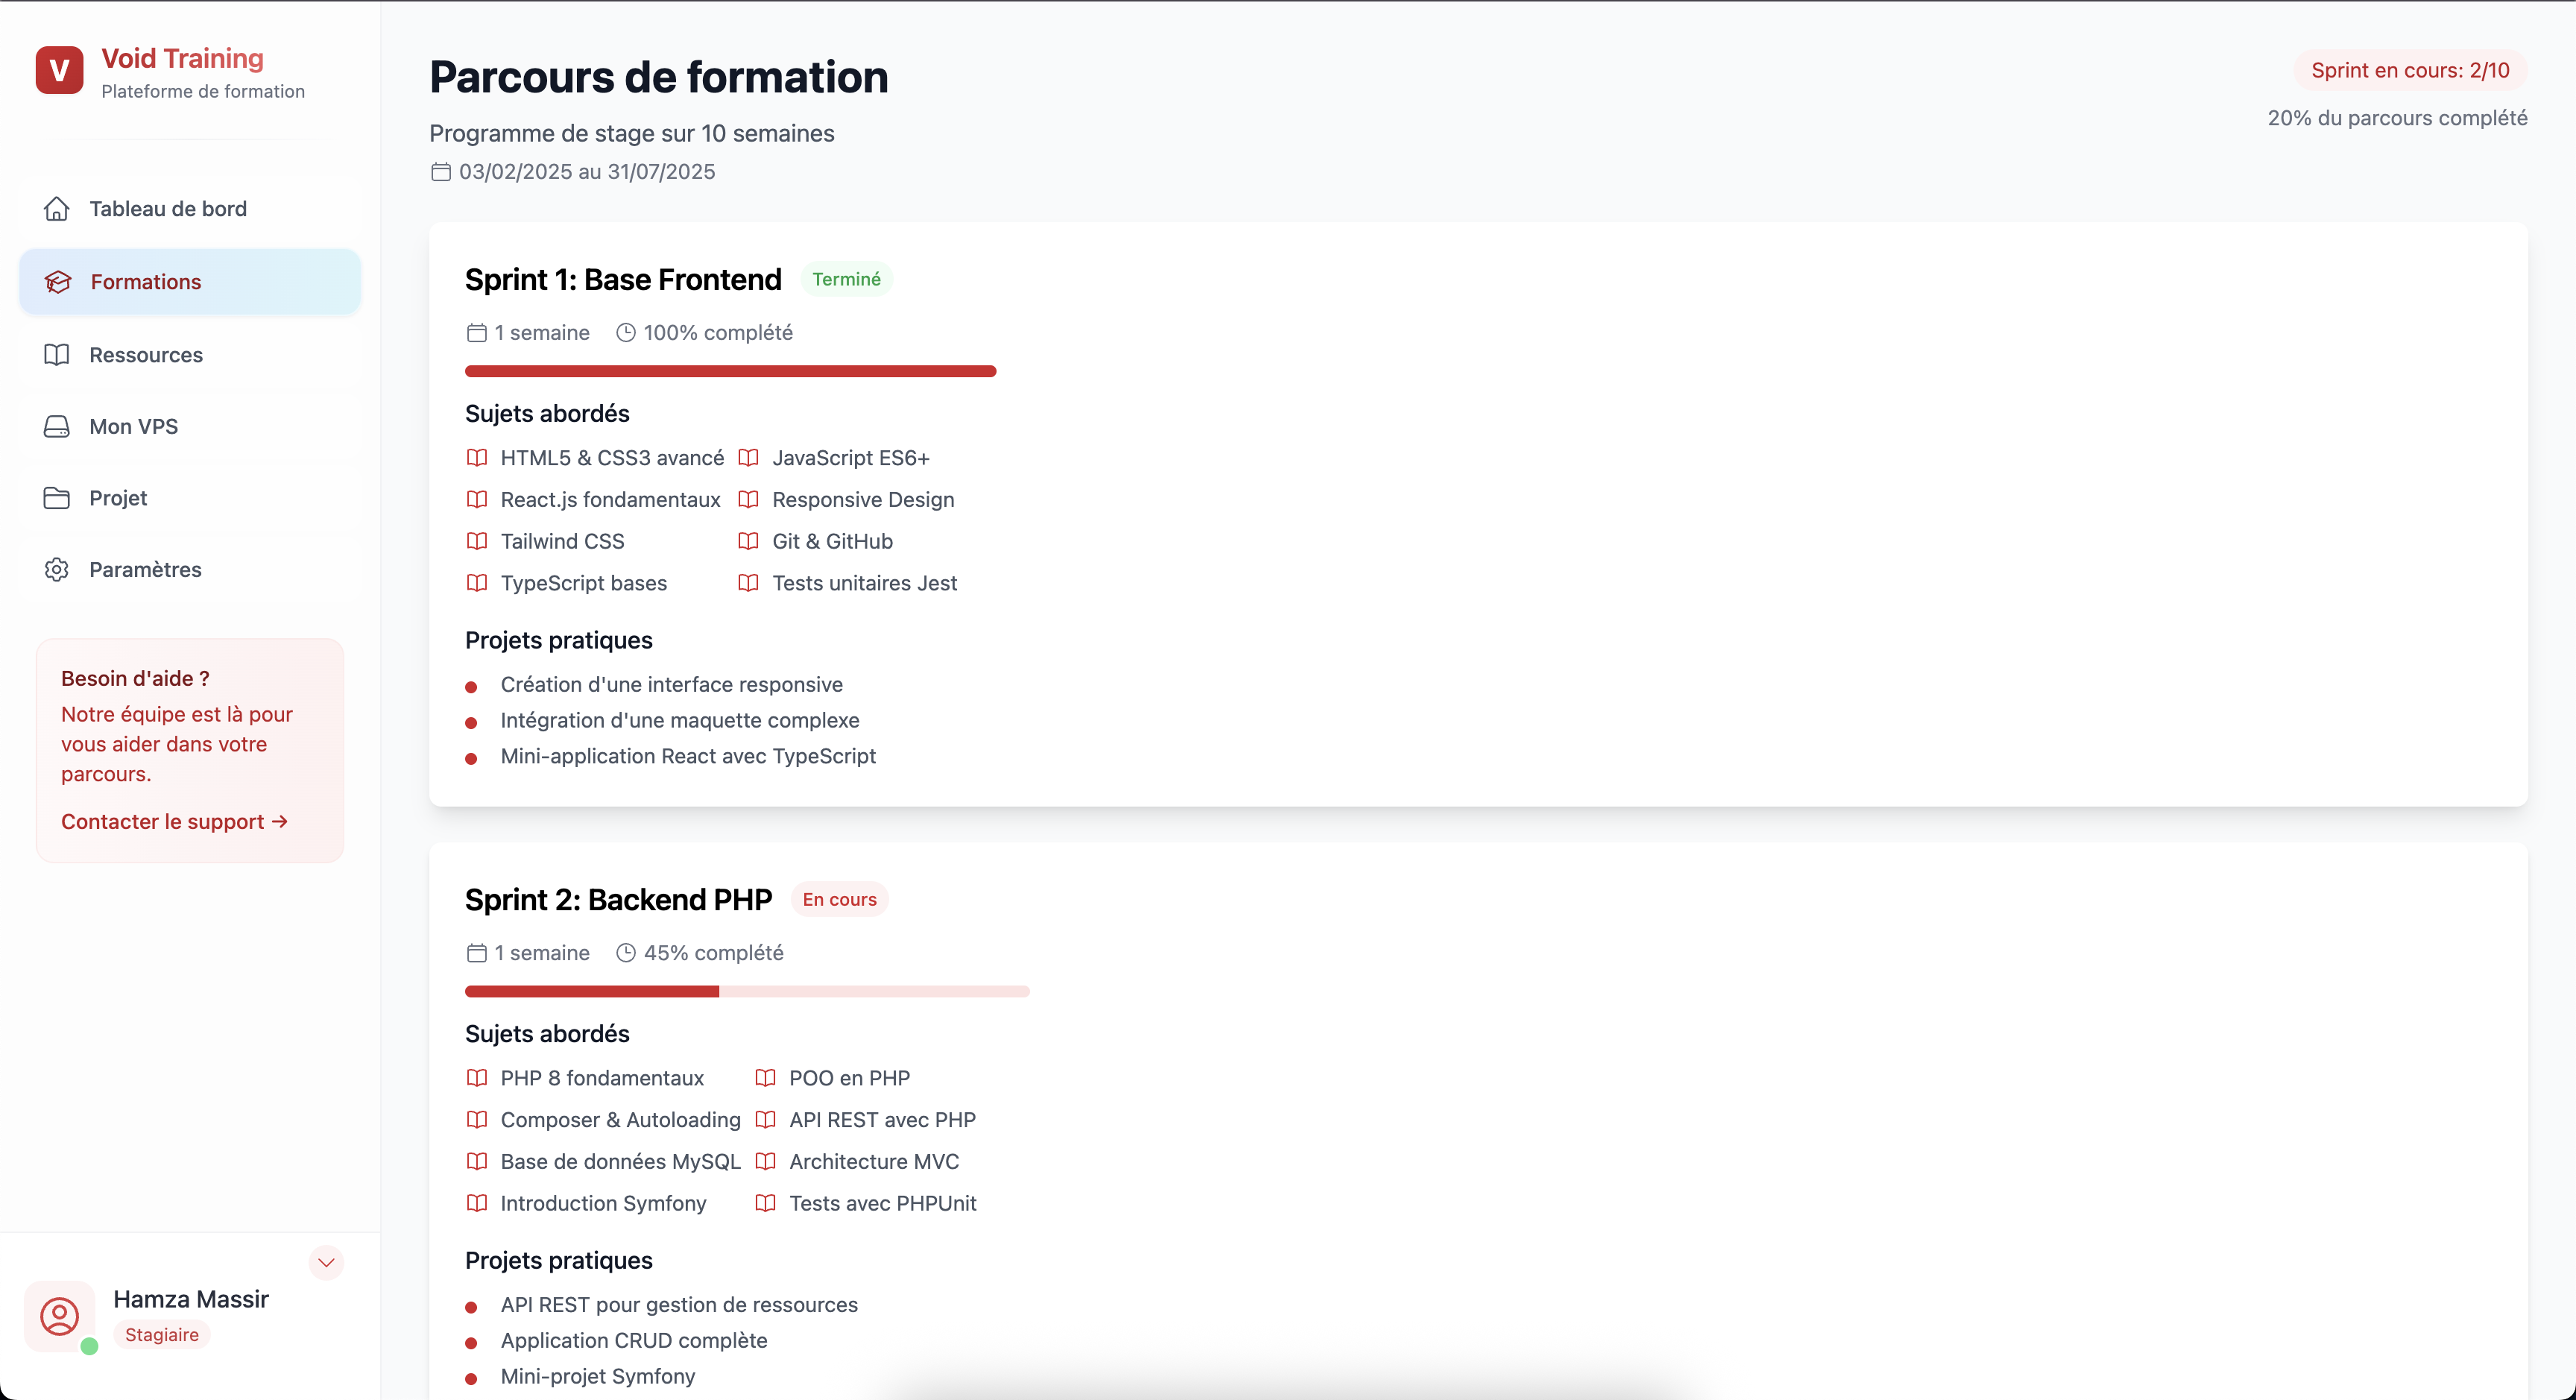
\includegraphics[width=1.1\textwidth]{images/Screenshot-intern-sprint-collection}%
    }
    \caption{Intern Sprint Listing}
    \label{fig:sprint_listing}
\end{figure}

The sprint listing shows:
\begin{itemize}
    \item All assigned sprints
    \item Current progress status
    \item Start and end dates
    \item Completion percentage
\end{itemize}

\begin{figure}[H]
    \centering
    \makebox[\textwidth]{%
        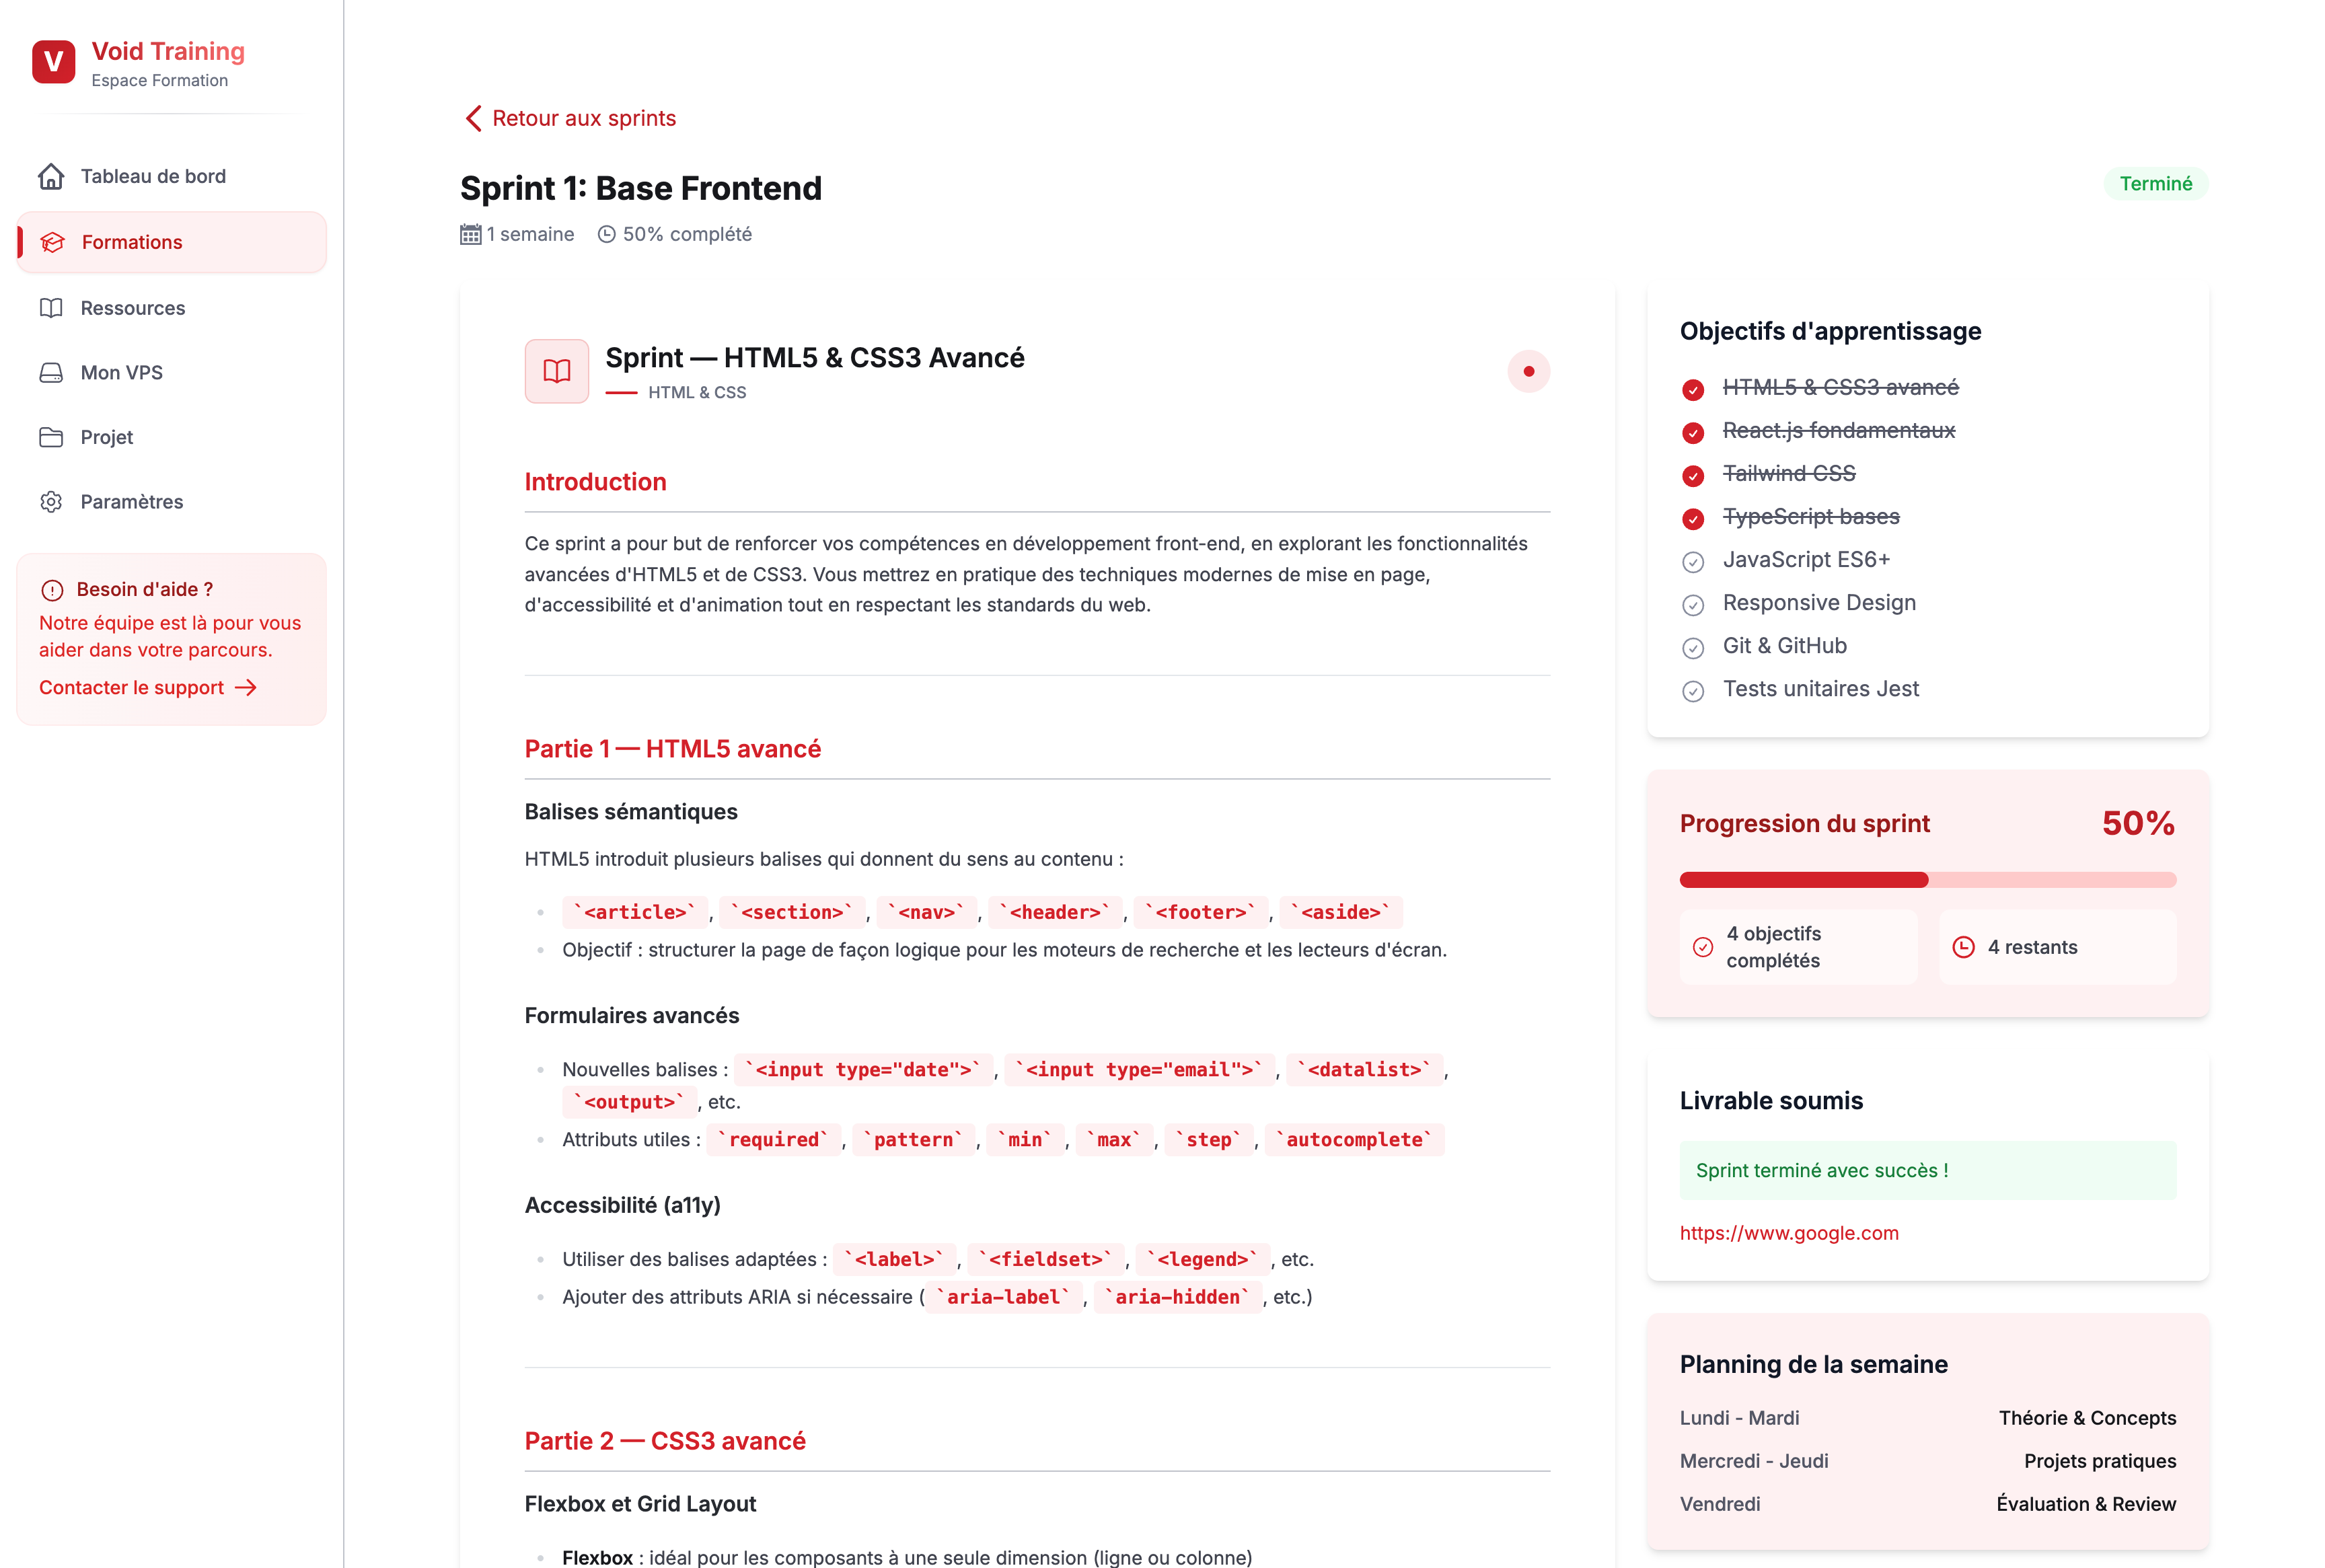
\includegraphics[width=1.1\textwidth]{images/screencapture-intern-sprint}%
    }
    \caption{Sprint Details Page}
    \label{fig:sprint_details}
\end{figure}

Each sprint page includes:
\begin{itemize}
    \item Learning objectives with progress tracking
    \item Clear deadlines for each task
    \item Required resources and materials
    \item Supervisor feedback section
\end{itemize}

\subsection{Learning Resources}
\noindent
A dedicated resources page provides additional learning materials:

\begin{figure}[H]
    \centering
    \makebox[\textwidth]{%
        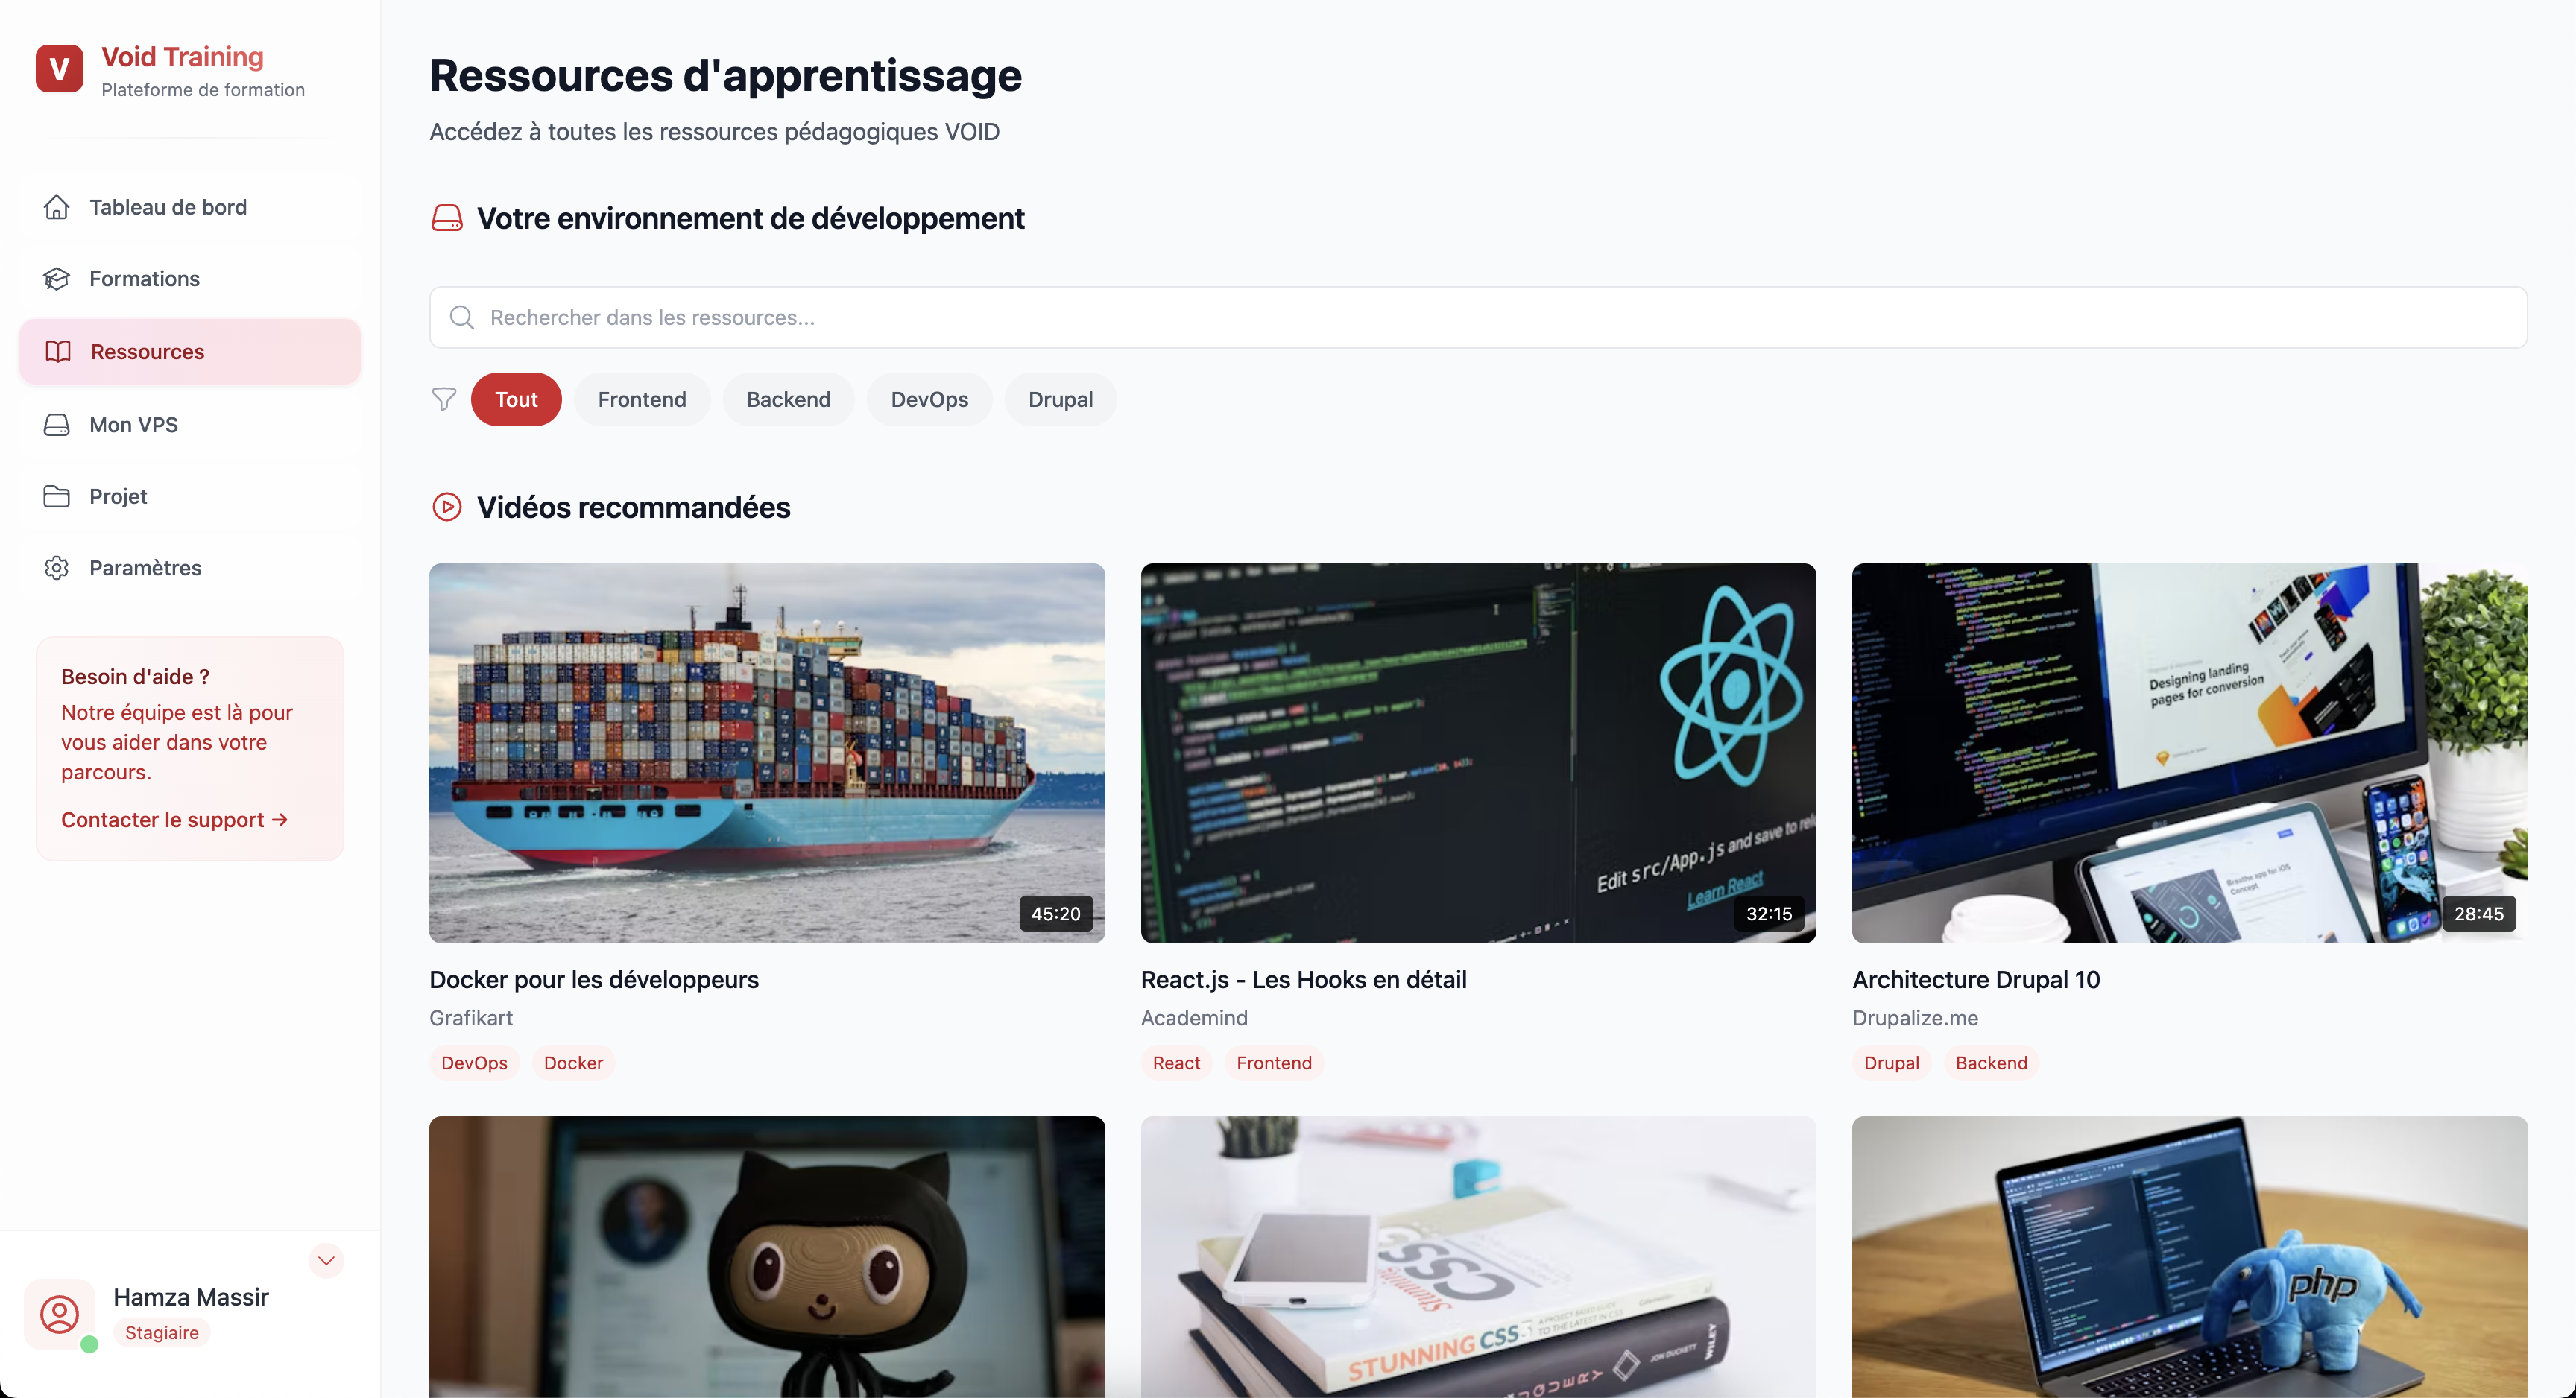
\includegraphics[width=1.1\textwidth]{images/Screenshot-intern-resources}%
    }
    \caption{Learning Resources Page}
    \label{fig:resources}
\end{figure}

\begin{figure}[H]
    \centering
    \makebox[\textwidth]{%
        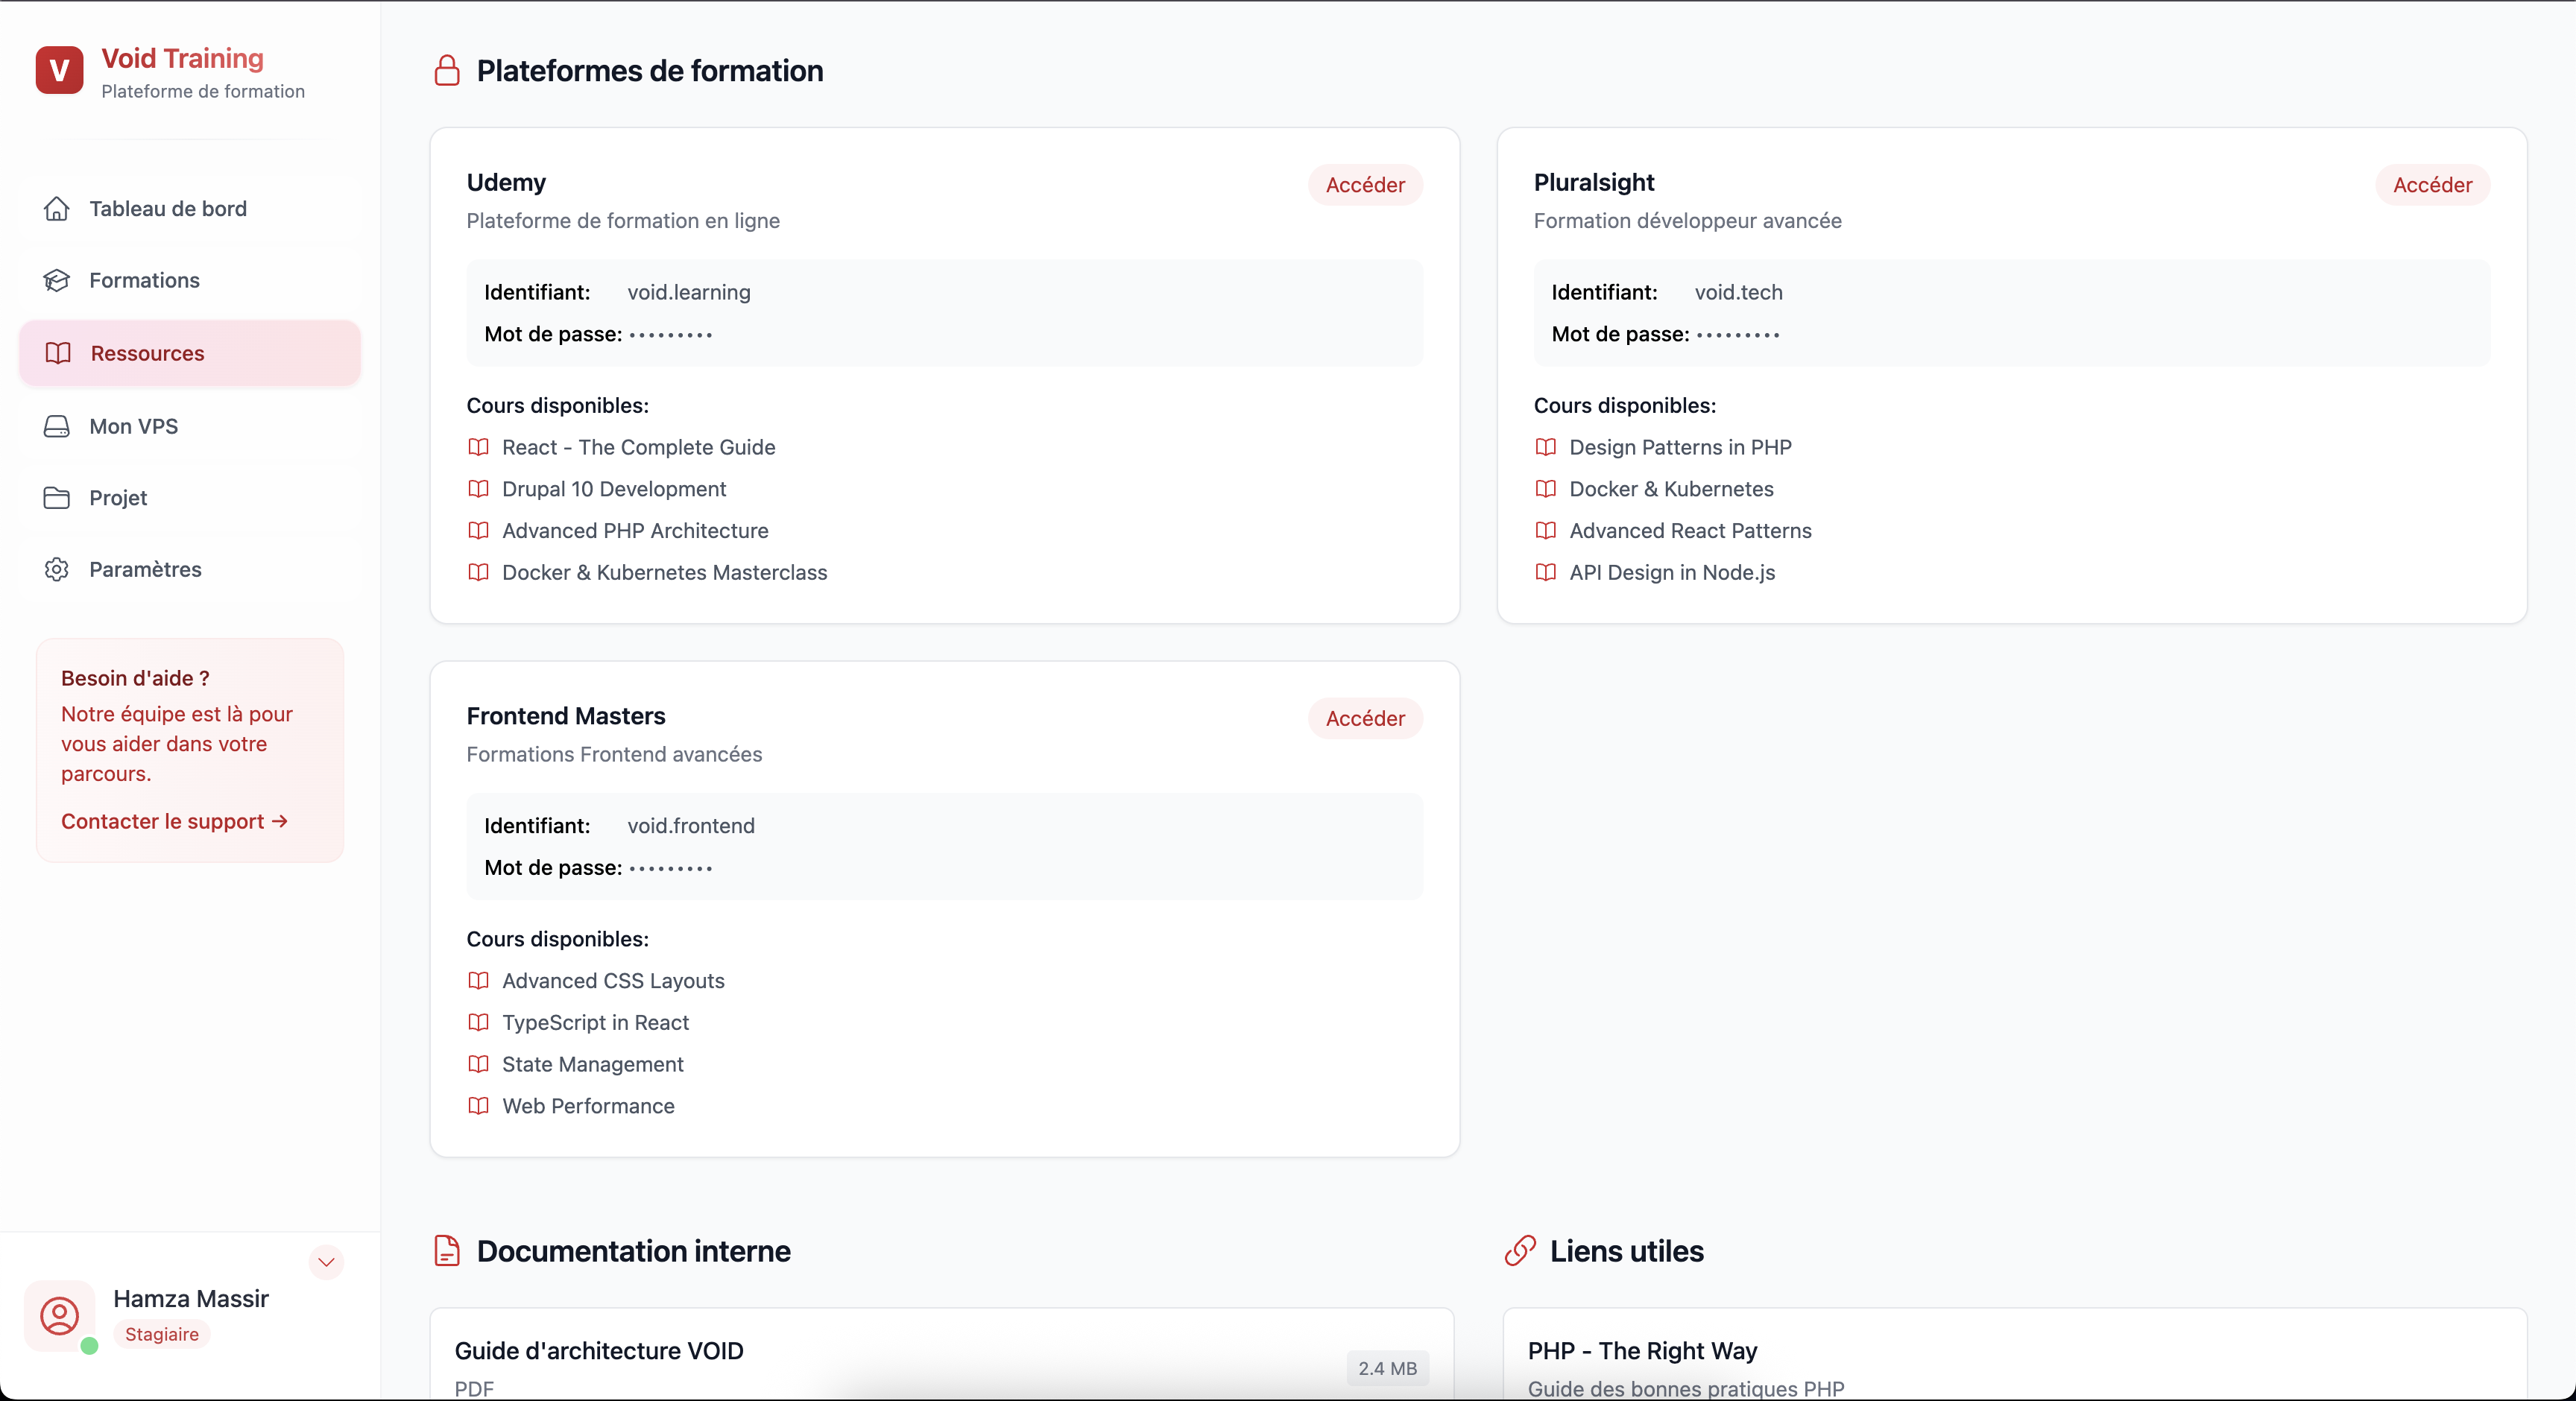
\includegraphics[width=1.1\textwidth]{images/Screenshot-intern-resources-accounts}%
    }
    \caption{Learning Resources Page (Accounts)}
    \label{fig:resources}
\end{figure}

The resources section offers:
\begin{itemize}
    \item Technical documentation
    \item Tutorial videos
    \item Code examples
    \item Best practices guides
\end{itemize}

\subsection{Project Management}
\noindent
Each intern has a dedicated project page:

\begin{figure}[H]
    \centering
    \makebox[\textwidth]{%
        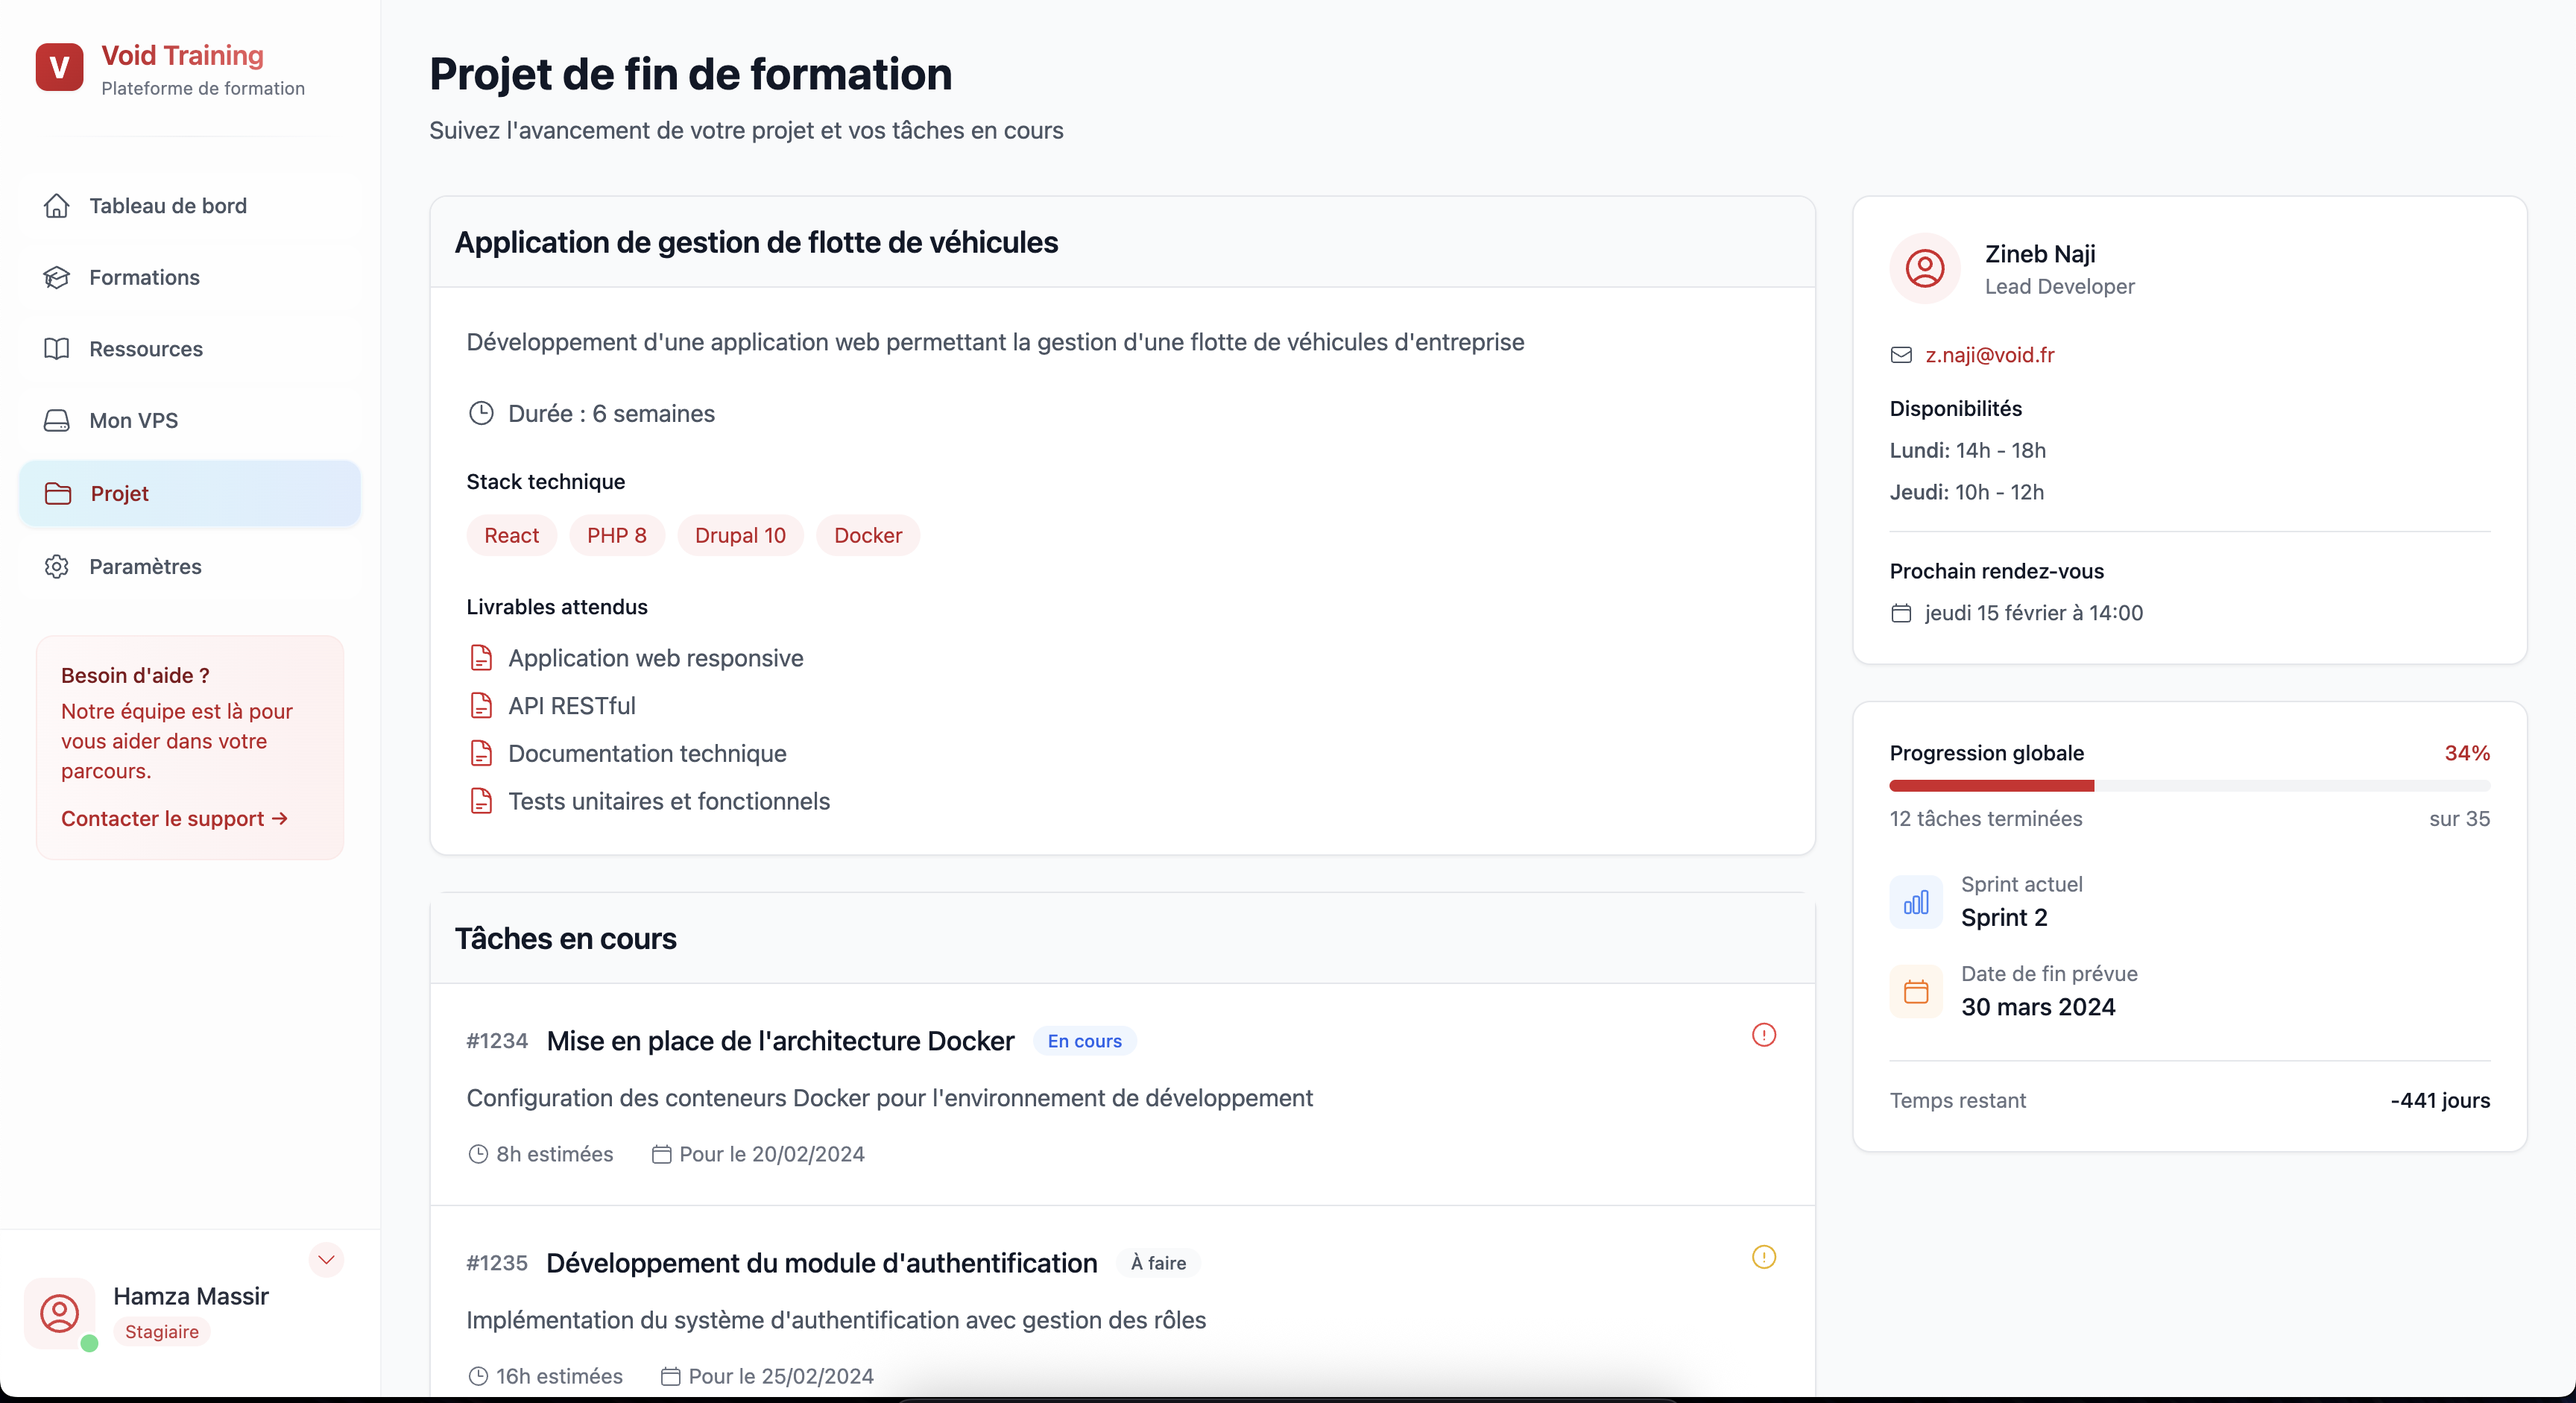
\includegraphics[width=1.1\textwidth]{images/Screenshot-project}%
    }
    \caption{Project Management Page}
    \label{fig:project}
\end{figure}

The project page shows:
\begin{itemize}
    \item Project requirements and goals
    \item Timeline and milestones
    \item Technical stack details
    \item Progress updates
    \item Supervisor comments
\end{itemize}

\subsection{User Profile}
\noindent
Interns can manage their personal information:

\begin{figure}[H]
    \centering
    \makebox[\textwidth]{%
        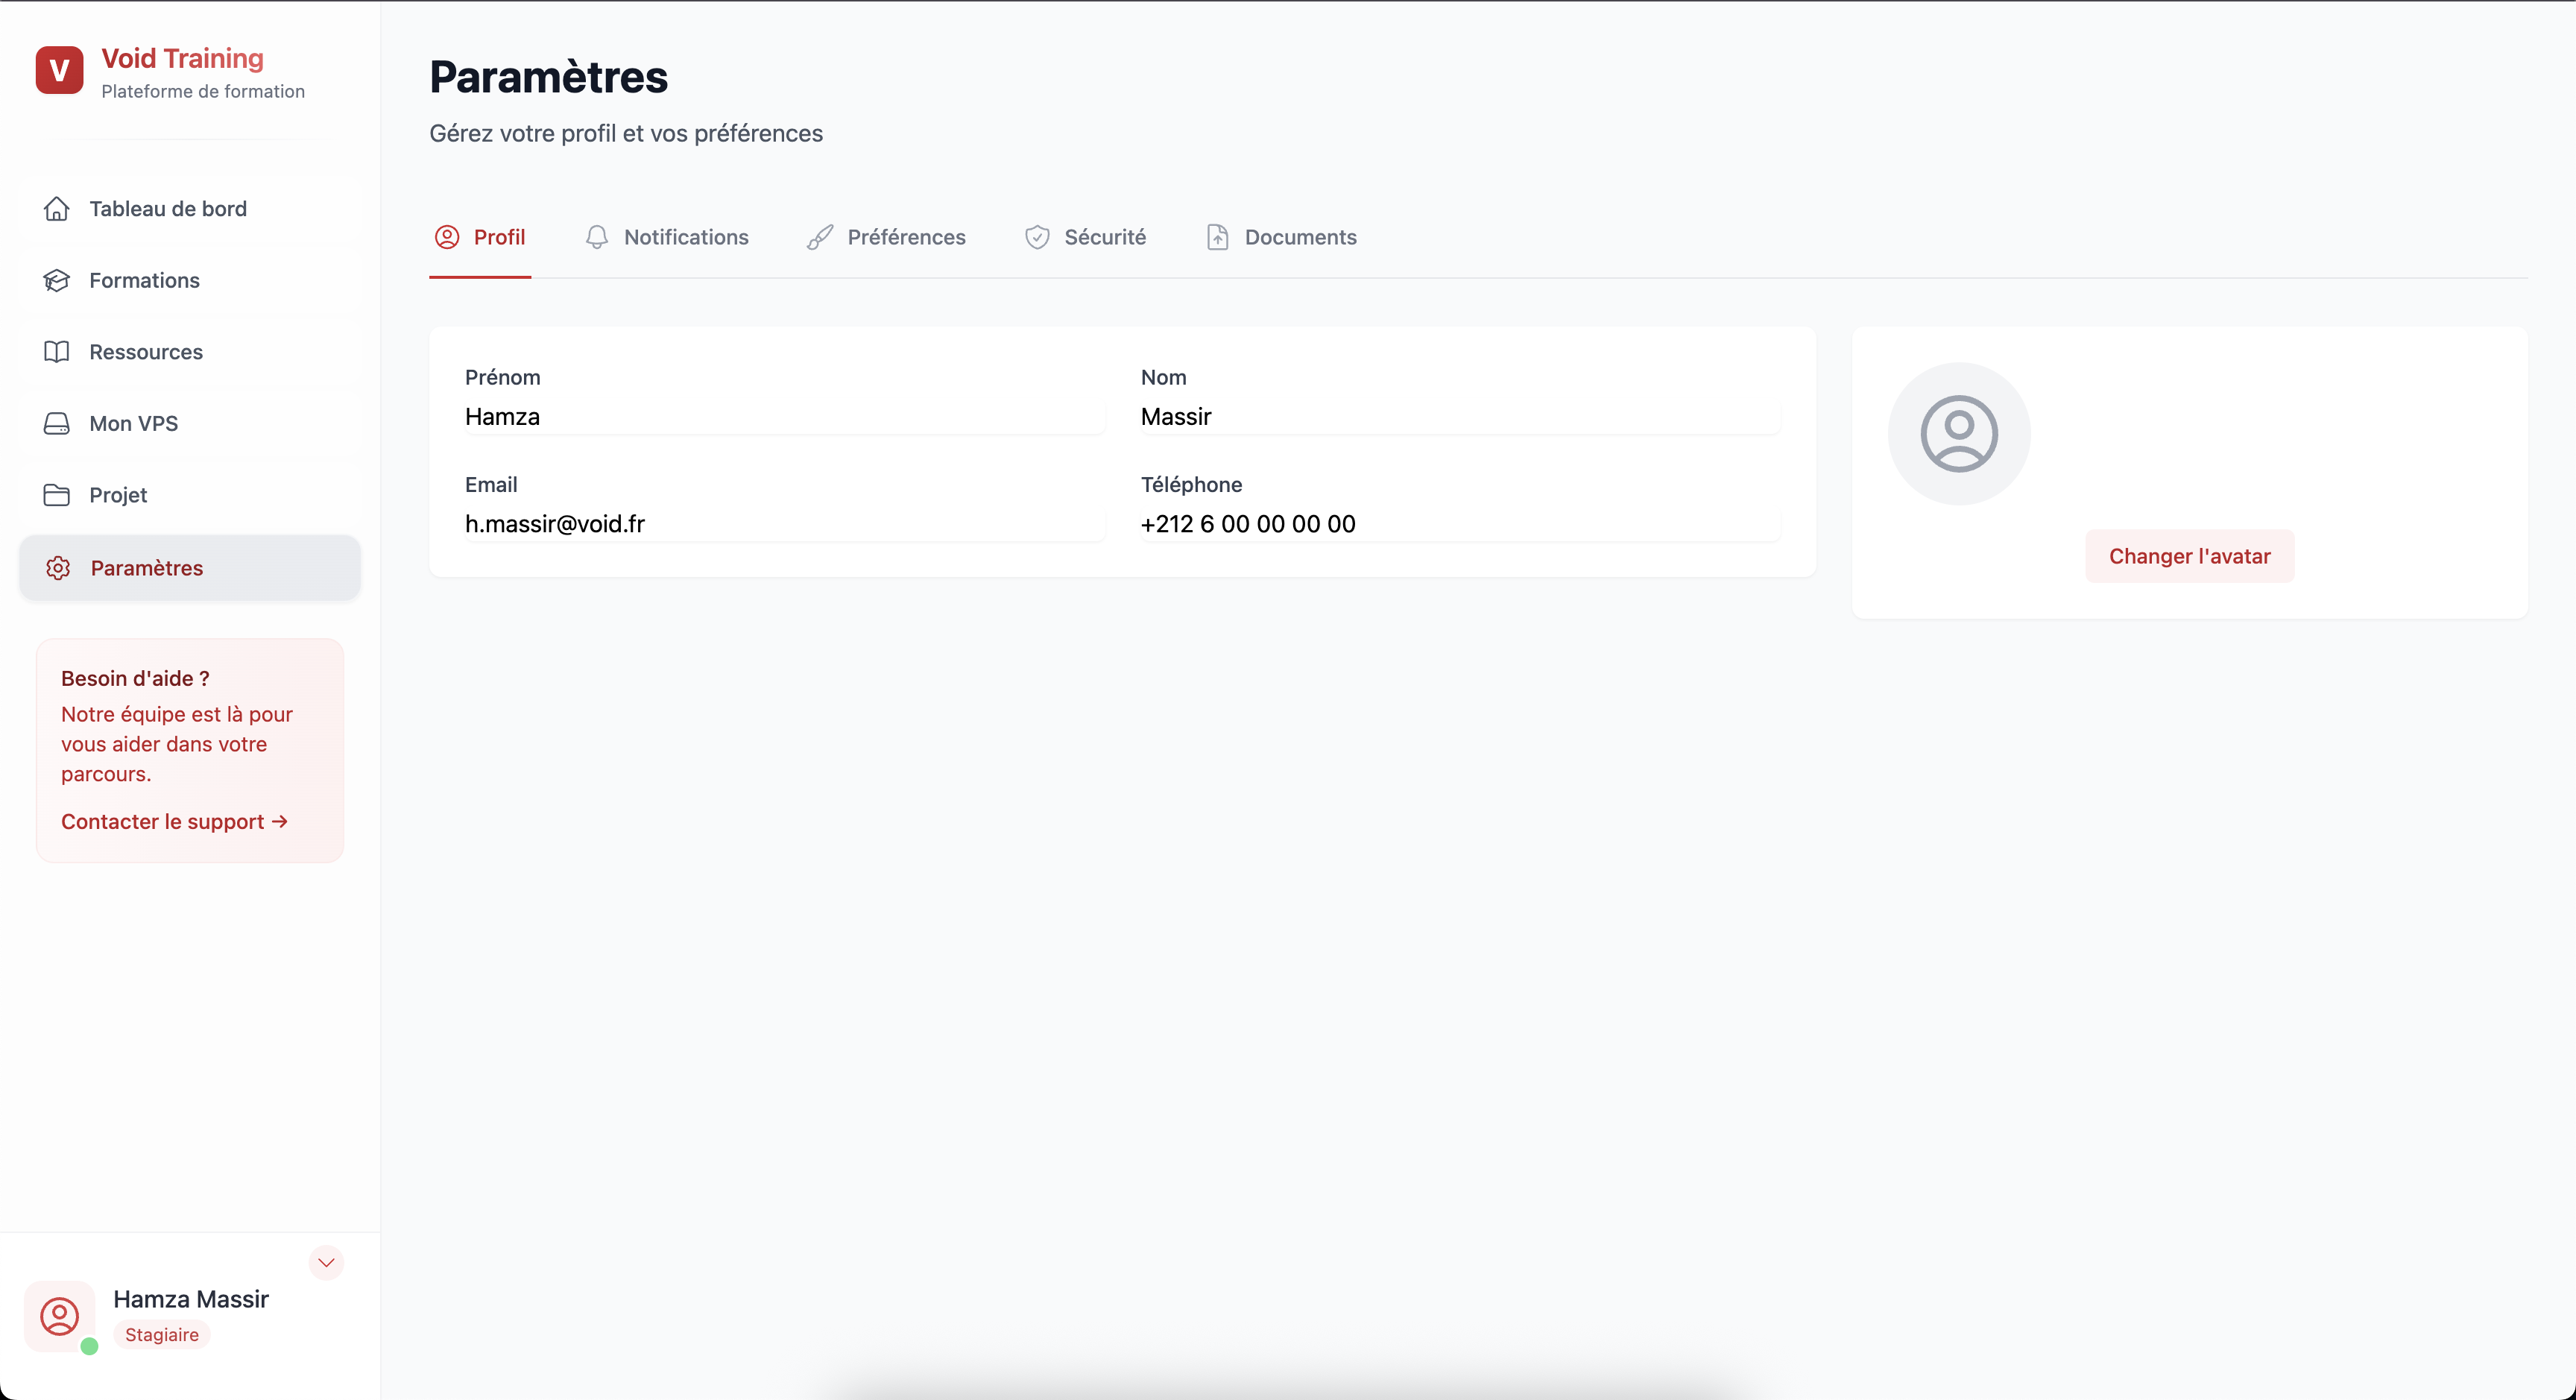
\includegraphics[width=1.1\textwidth]{images/Screenshot-intern-profil}%
    }
    \caption{User Profile Page}
    \label{fig:profile}
\end{figure}

The profile page allows:
\begin{itemize}
    \item Update personal information
    \item Change profile picture
    \item View application history
    \item Access personal documents
\end{itemize}

\subsection{Document Management}
\noindent
A secure space for personal documents:

\begin{figure}[H]
    \centering
    \makebox[\textwidth]{%
        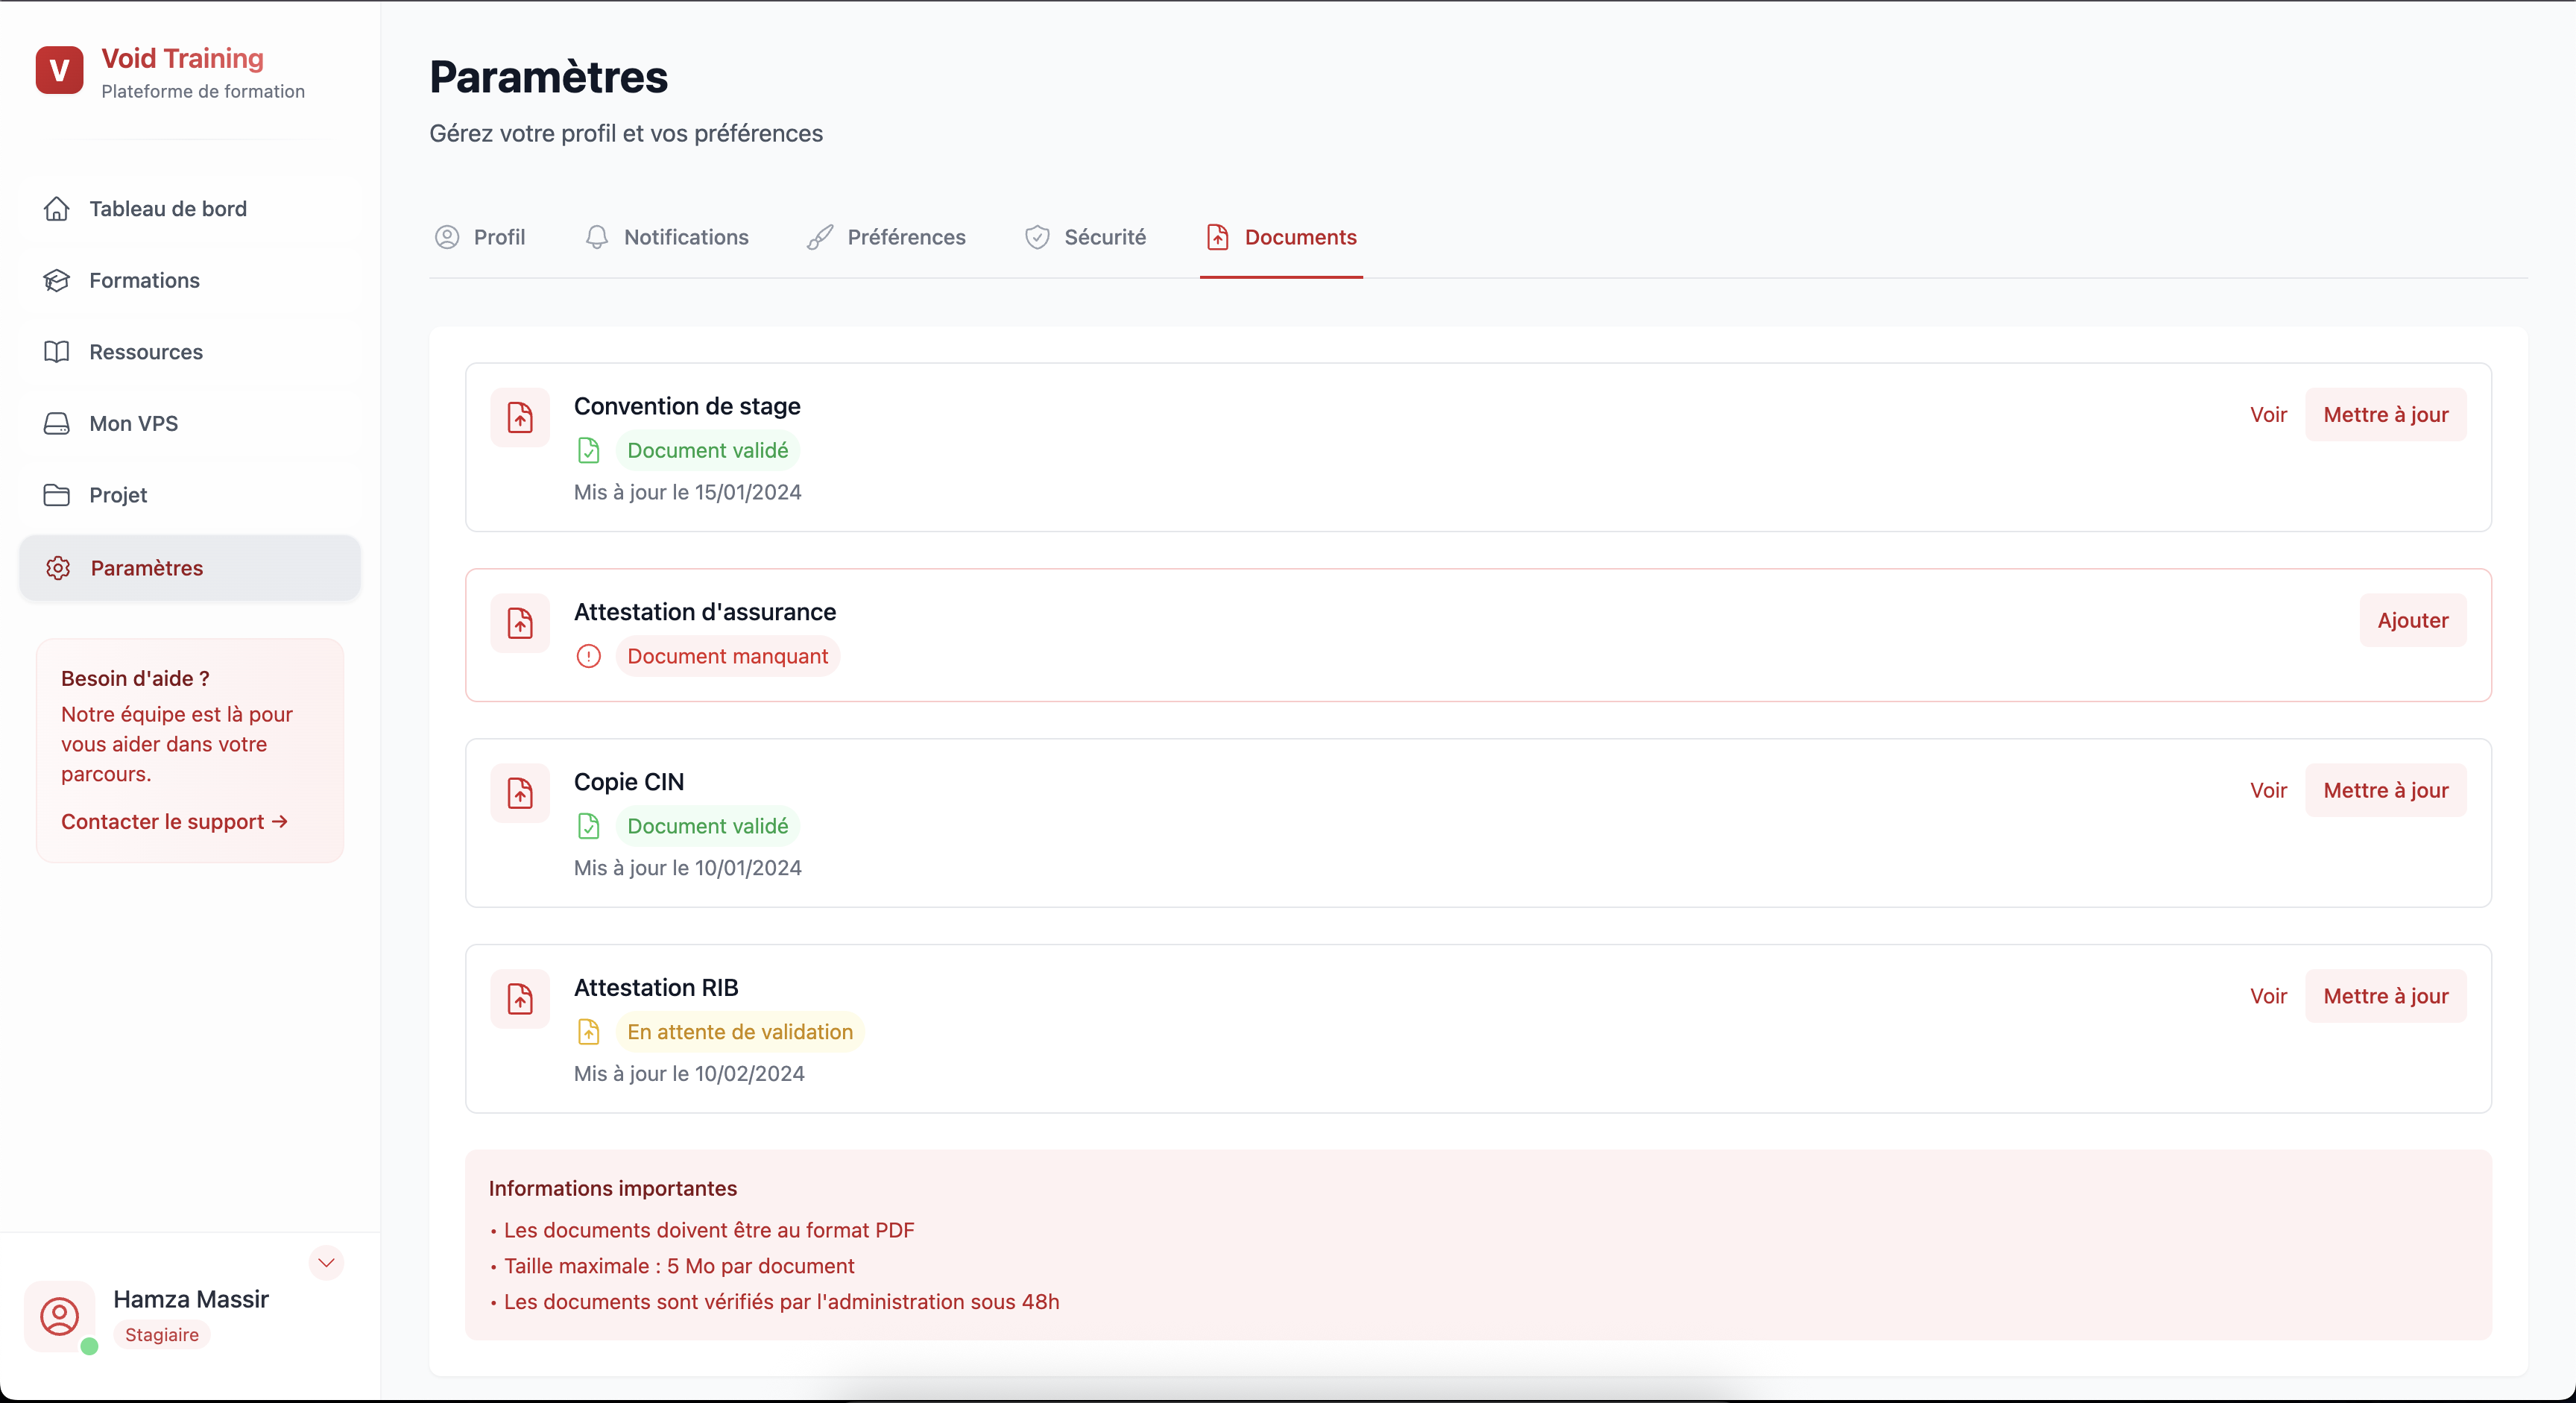
\includegraphics[width=1.1\textwidth]{images/Screenshot-intern-documents}%
    }
    \caption{Document Management Page}
    \label{fig:documents}
\end{figure}

The documents section provides:
\begin{itemize}
    \item Upload and download files
    \item View document history
    \item Share documents with supervisors
    \item Track document status
\end{itemize}

\subsection{Project Deployment}
\noindent
The deployment of the Candidate Platform was streamlined through an automated CI/CD pipeline integrated with Bitbucket. The deployment process is triggered automatically upon each tagged commit, ensuring consistent and reliable releases. The production environment leverages containerized services with Traefik handling SSL certificate management and load balancing, while Nginx serves as a reverse proxy for the frontend application.

\subsubsection{Production Architecture Overview}
The production environment implements a multi-layered architecture designed for scalability, security, and performance:

\begin{itemize}
    \item \textbf{External User Layer}: Users access the platform through standard HTTP/HTTPS requests via web browsers to the public domain.
    
    \item \textbf{Edge Router (Traefik)}: Acts as the primary entry point, performing SSL termination using Let's Encrypt certificates and implementing container-based routing rules to direct traffic to appropriate services.
    
    \item \textbf{Reverse Proxy (Nginx)}: Handles request caching and forwards uncached requests to the Next.js frontend container, optimizing response times for static content.
    
    \item \textbf{Frontend Application (Next.js)}: Serves the user interface, rendering static pages and managing client-side interactions while communicating with the backend through JSON:API endpoints.
    
    \item \textbf{Backend API (Drupal)}: Processes business logic, handles authentication, and manages data operations through a headless CMS architecture.
    
    \item \textbf{Database Layer (MySQL)}: Provides persistent data storage and retrieval for all application data and user information.
\end{itemize}

\subsubsection{Performance Optimization Strategy}
To ensure optimal performance and minimal latency, the platform implements a multi-tier caching strategy:

\begin{itemize}
    \item \textbf{Frontend Caching (Redis)}: The frontend container utilizes Redis as a high-performance key-value store for user sessions and temporary application state, reducing authentication overhead.
    
    \item \textbf{Backend Caching (Memcached)}: The backend container employs Memcached to cache database query results, significantly reducing database load and improving response times for frequently accessed data.
    
    \item \textbf{Caching Layer Separation}: Redis and Memcached operate independently, serving distinct optimization purposes - frontend user experience optimization versus backend data access optimization.
\end{itemize}

\begin{figure}[H]
    \centering
    \makebox[\textwidth]{%
        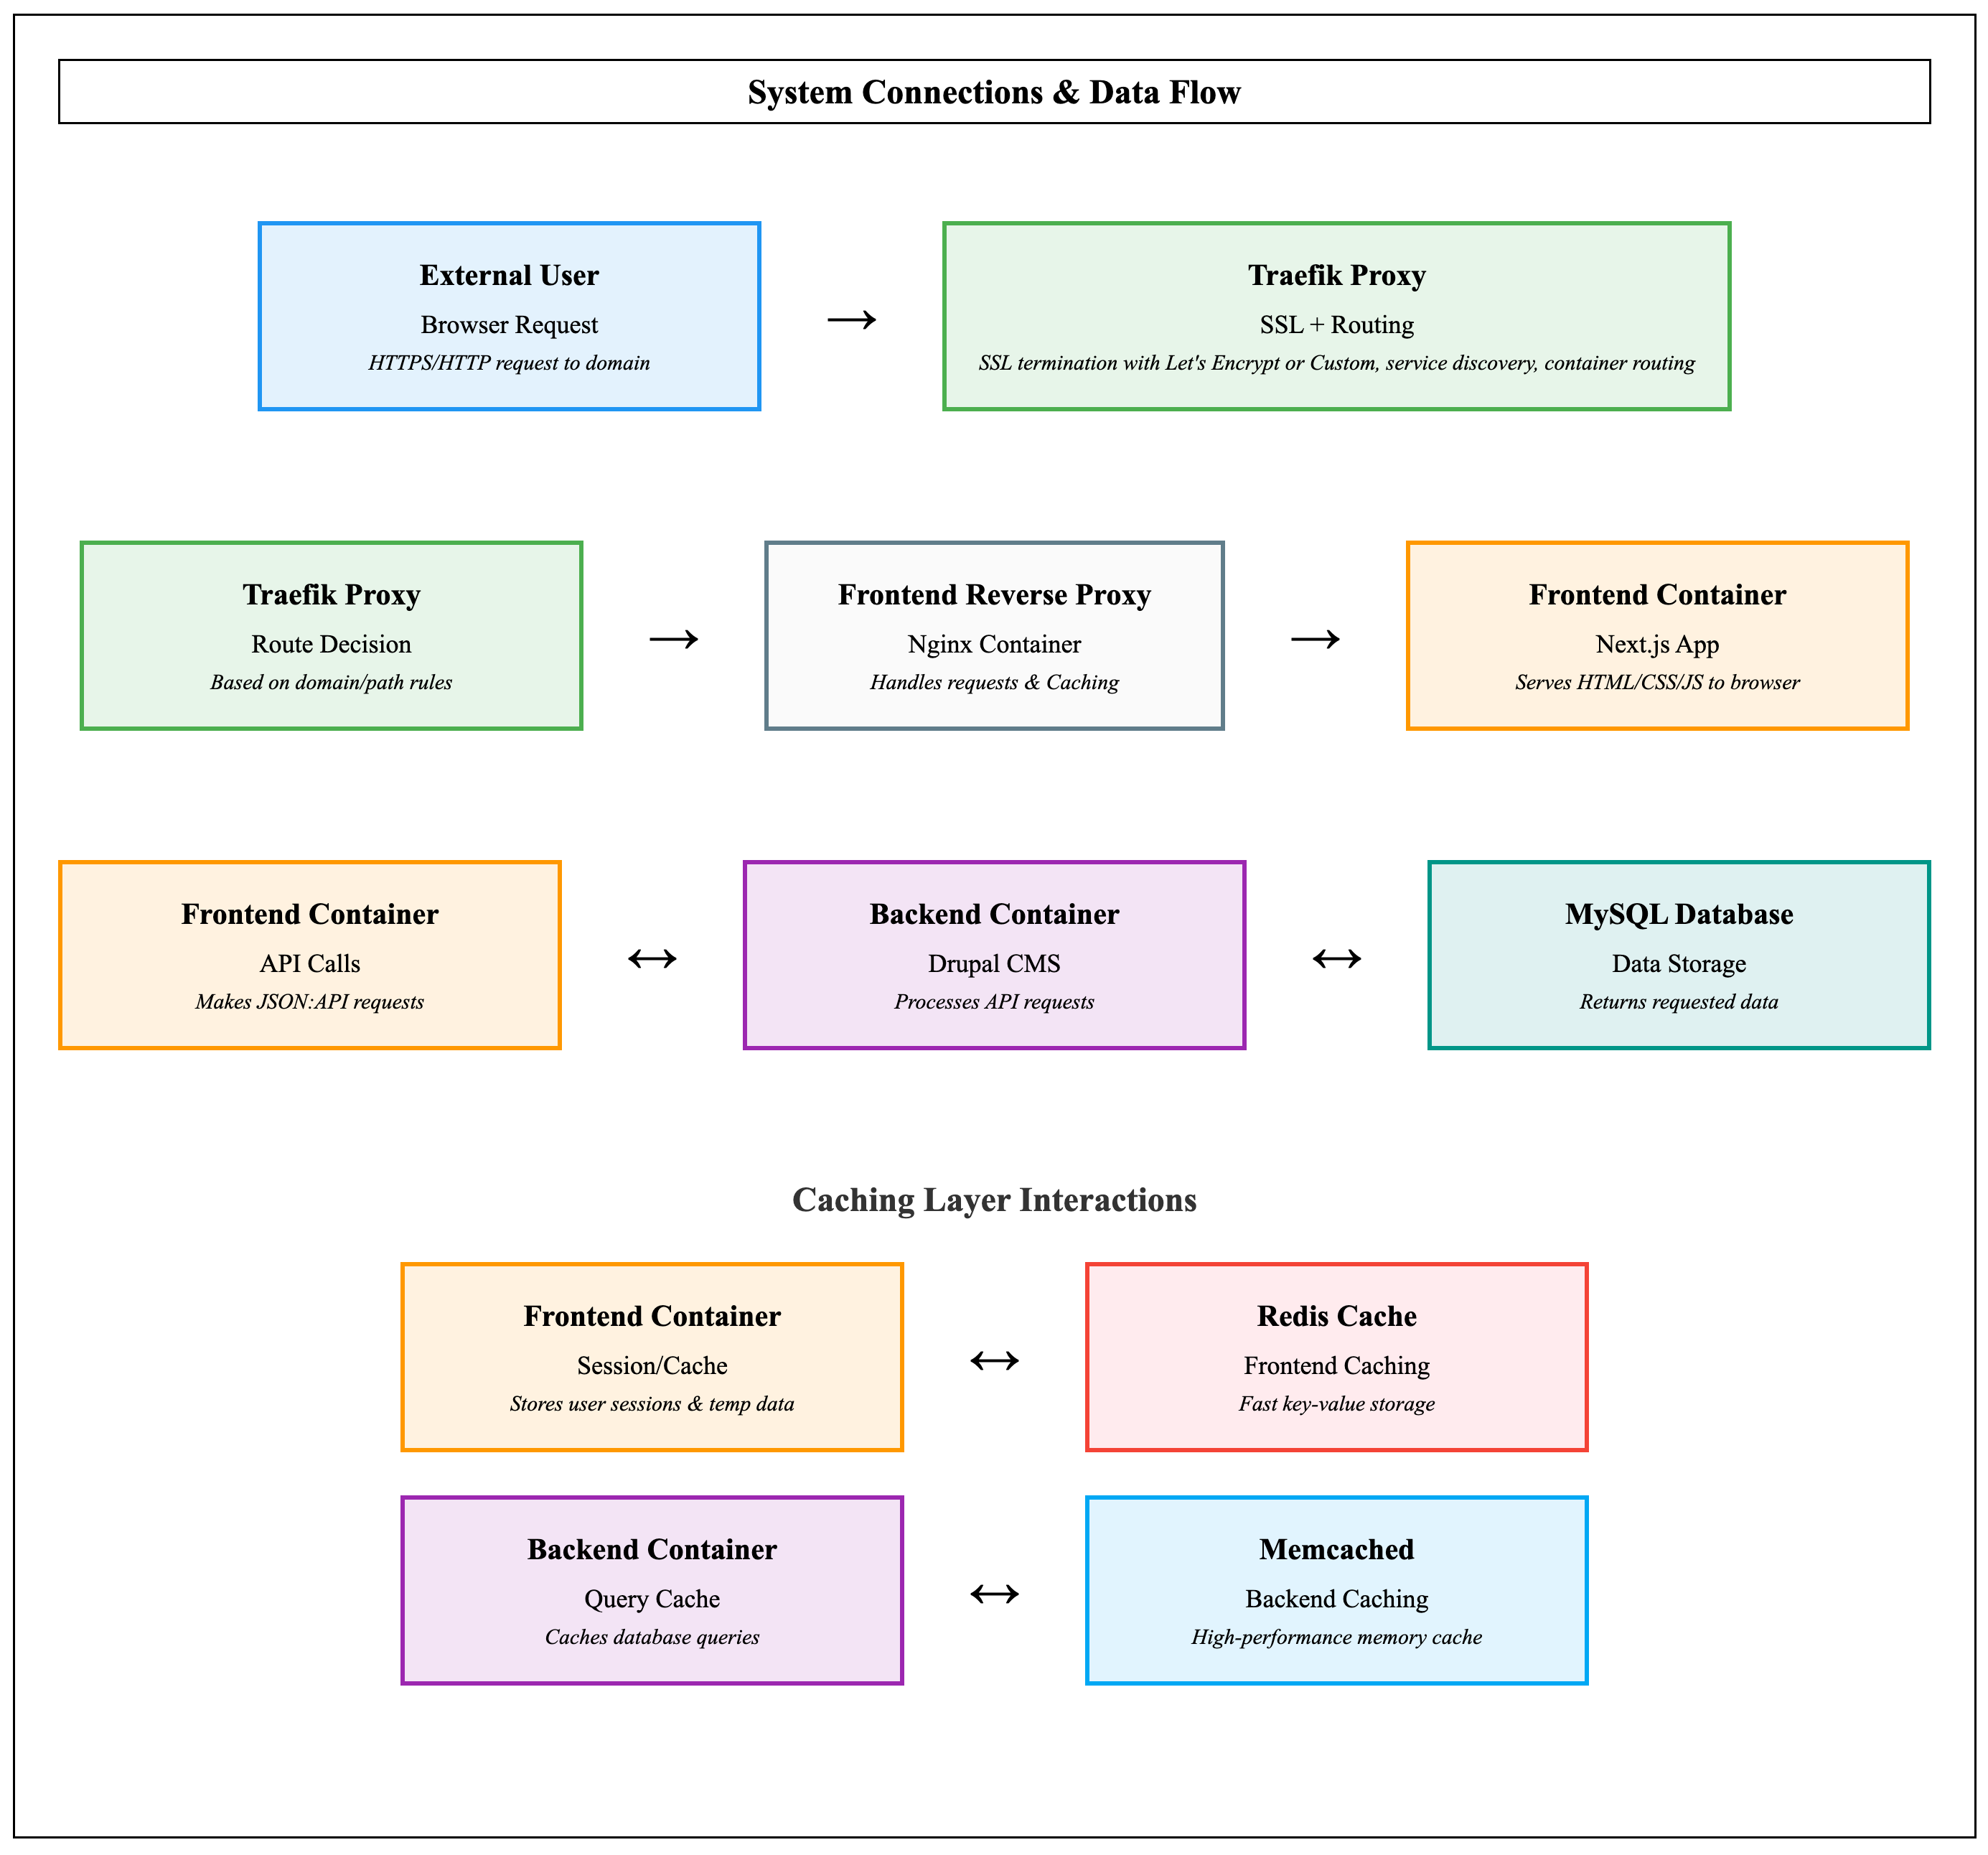
\includegraphics[width=1.1\textwidth]{images/prodStructure.png}%
    }
    \caption{Production Environment Architecture}
    \label{fig:production_architecture}
\end{figure}

\subsection{Conclusion}
\noindent
The Candidate Platform has successfully transformed VOID Digital Agency's intern recruitment process into a more efficient, transparent, and scalable system. Through the implementation of automated workflows, structured evaluation processes, and clear communication channels, the platform has significantly enhanced the overall recruitment experience for both candidates and recruiters. The robust production architecture ensures reliable performance, security, and maintainability, providing a solid foundation for future enhancements and scaling requirements.
